\documentclass[12pt,a4paper]{report}

\usepackage[utf8]{inputenc} % pentru suport diacritice
\usepackage[T1]{fontenc}    % codificare fonturi — redare corectă ș/ț
\usepackage[romanian]{babel} % setări pentru limba română
\renewcommand\familydefault{\sfdefault} % sans serif

\usepackage[margin=2.54cm]{geometry}	% dimensiuni pagină și margini
\usepackage{graphicx} % support the \includegraphics command and options

% formatting sections and subsections
\usepackage{textcase}
\usepackage[titletoc, title]{appendix}
\usepackage{titlesec}
\titleformat{\chapter}{\large\bfseries\MakeUppercase}{\thechapter}{2ex}{}[\vspace*{-1.5cm}]
\titleformat*{\section}{\large\bfseries}
\titleformat*{\subsection}{\large\bfseries}
\titleformat*{\subsubsection}{\large\bfseries}

\usepackage{chngcntr}
\counterwithout{figure}{chapter} % no chapter number in figure labels
\counterwithout{table}{chapter} % no chapter number in table labels
\counterwithout{equation}{chapter} % no chapter number in equation labels

\usepackage{booktabs} % for much better looking tables
\usepackage{url} % Useful for inserting web links nicely
\usepackage[bookmarks,unicode,hidelinks]{hyperref}

\usepackage{array} % for better arrays (eg matrices) in maths
\usepackage{paralist} % very flexible & customisable lists (eg. enumerate/itemize, etc.)
\usepackage{verbatim} % adds environment for commenting out blocks of text & for better verbatim
\usepackage{subfig} % make it possible to include more than one captioned figure/table in a single float
\usepackage{enumitem}
\setlist{noitemsep}

%%% HEADERS & FOOTERS
\usepackage{fancyhdr}
\pagestyle{empty}
\renewcommand{\headrulewidth}{0pt}
\renewcommand{\footrulewidth}{0pt}
\lhead{}\chead{}\rhead{}
\lfoot{}\cfoot{\thepage}\rfoot{}

%%%%%%%%%%%%%%%%%%%%%%%%%%%%%%%%%%%%%%%%%%%%%%%%%%
%%   Pachete adăugate pentru această lucrare
%%%%%%%%%%%%%%%%%%%%%%%%%%%%%%%%%%%%%%%%%%%%%%%%%%
\usepackage{xcolor}
\usepackage{listings}

% ── Stil pentru secvențele de cod JavaScript/Node.js ──
\definecolor{codekw}{RGB}{0,51,153}
\definecolor{codestr}{RGB}{163,21,21}
\definecolor{codecomment}{RGB}{0,128,0}
\definecolor{codebg}{RGB}{248,248,248}
\definecolor{coderule}{RGB}{200,200,200}

\lstdefinelanguage{JavaScript}{
  keywords={typeof, new, true, false, catch, function, return, null, undefined,
            switch, var, if, in, while, do, else, case, break, const, let,
            await, async, this, of, for, try, throw, delete, continue},
  keywordstyle=\color{codekw}\bfseries,
  ndkeywords={class, export, extends, import, require, module},
  ndkeywordstyle=\color{codekw}\bfseries,
  identifierstyle=\color{black},
  sensitive=true,
  comment=[l]{//},
  morecomment=[s]{/*}{*/},
  commentstyle=\color{codecomment}\itshape,
  stringstyle=\color{codestr},
  morestring=[b]',
  morestring=[b]",
  morestring=[b]`
}

\lstset{
  language=JavaScript,
  basicstyle=\ttfamily\footnotesize,
  numbers=left,
  numberstyle=\tiny\color{gray},
  numbersep=8pt,
  breaklines=true,
  breakatwhitespace=true,
  frame=single,
  rulecolor=\color{coderule},
  backgroundcolor=\color{codebg},
  tabsize=2,
  showstringspaces=false,
  captionpos=b,
  aboveskip=10pt,
  belowskip=6pt,
  literate=%
    {ă}{{\u{a}}}1 {Ă}{{\u{A}}}1
    {â}{{\^{a}}}1 {Â}{{\^{A}}}1
    {î}{{\^{\i}}}1 {Î}{{\^{I}}}1
    {ș}{{\textcommabelow{s}}}1 {Ș}{{\textcommabelow{S}}}1
    {ț}{{\textcommabelow{t}}}1 {Ț}{{\textcommabelow{T}}}1
    {ş}{{\c{s}}}1 {Ş}{{\c{S}}}1
    {ţ}{{\c{t}}}1 {Ţ}{{\c{T}}}1
    {—}{{---}}2 {–}{{--}}1
    {„}{{,,}}1 {”}{{''}}1 {’}{{'}}1 {…}{{...}}2
    {≥}{{$\geq$}}1 {≤}{{$\leq$}}1 {→}{{$\to$}}1 {←}{{$\gets$}}1
}
\renewcommand{\lstlistingname}{Cod}

% ── Marcaje vizibile pentru elementele de completat de către autor ──
% [TODO: ...] apare cu roșu în PDF — ușor de găsit înainte de predare.
\newcommand{\todoinline}[1]{\textcolor{red}{\textbf{[TODO: #1]}}}
% Valoare numerică ce trebuie măsurată/completată în tabele.
\newcommand{\todoval}{\textcolor{red}{[de completat]}}

% ── Placeholder pentru figuri ───────────────────────────────────────
% Utilizare: \placeholderfig{<lățime 0..1>}{<nume-fișier-fără-extensie>}{<înălțime casetă>}{<ce trebuie să conțină>}{<caption>}
% Înlocuire: șterge \fbox{...} și decomentează linia \includegraphics.
\newcommand{\placeholderfig}[5]{%
  \begin{figure}[!ht]
    \centering
    % \includegraphics[width=#1\textwidth]{pics/#2}
    \fbox{\parbox[c][#3][c]{#1\textwidth}{\centering
      \textcolor{red}{\textbf{[DE ADĂUGAT: \texttt{pics/#2.png}]}}\\[8pt]
      {\small\itshape #4}}}
    \caption{#5}
    \label{fig:#2}
  \end{figure}
}

%%%%%%%%%%%%%%%%%%%%%%%%%%%%%%%%%%%%%%%%%%%%%%%%%%
%%   Macro-uri pagini de titlu (din template)
%%%%%%%%%%%%%%%%%%%%%%%%%%%%%%%%%%%%%%%%%%%%%%%%%%

\newcommand{\HeaderLineSpace}{-0.25cm}
\newcommand{\UniTextRO}{UNIVERSITATEA POLITEHNICA DIN BUCUREȘTI \\[\HeaderLineSpace]
FACULTATEA DE AUTOMATICĂ ȘI CALCULATOARE \\[\HeaderLineSpace]
DEPARTAMENTUL DE CALCULATOARE\\}
\newcommand{\DiplomaRO}{PROIECT DE DIPLOMĂ}
\newcommand{\AdvisorRO}{Coordonator științific:}
\newcommand{\BucRO}{BUCUREȘTI}

\newcommand{\UniTextEN}{UNIVERSITY POLITEHNICA OF BUCHAREST \\[\HeaderLineSpace]
FACULTY OF AUTOMATIC CONTROL AND COMPUTERS \\[\HeaderLineSpace]
COMPUTER SCIENCE AND ENGINEERING DEPARTMENT\\}
\newcommand{\DiplomaEN}{DIPLOMA PROJECT}
\newcommand{\AdvisorEN}{Thesis advisor:}
\newcommand{\BucEN}{BUCHAREST}

\newcommand{\frontPage}[6]{
\begin{titlepage}
\begin{center}
{\Large #1}  % header (university, faculty, department)
\vspace{50pt}
\begin{tabular}{p{6cm}p{4cm}}
% Logo-urile provin din template-ul oficial; dacă lipsesc, se afișează
% casete placeholder ca documentul să compileze oricum.
\IfFileExists{pics/upb-logo.jpg}%
  {
\includegraphics[scale=0.8]{pics/upb-logo.jpg}}%
  {\fbox{\parbox[c][2.8cm][c]{4.5cm}{\centering\small [pics/upb-logo.jpg]}}} &
	\IfFileExists{pics/cs-logo.pdf}%
  {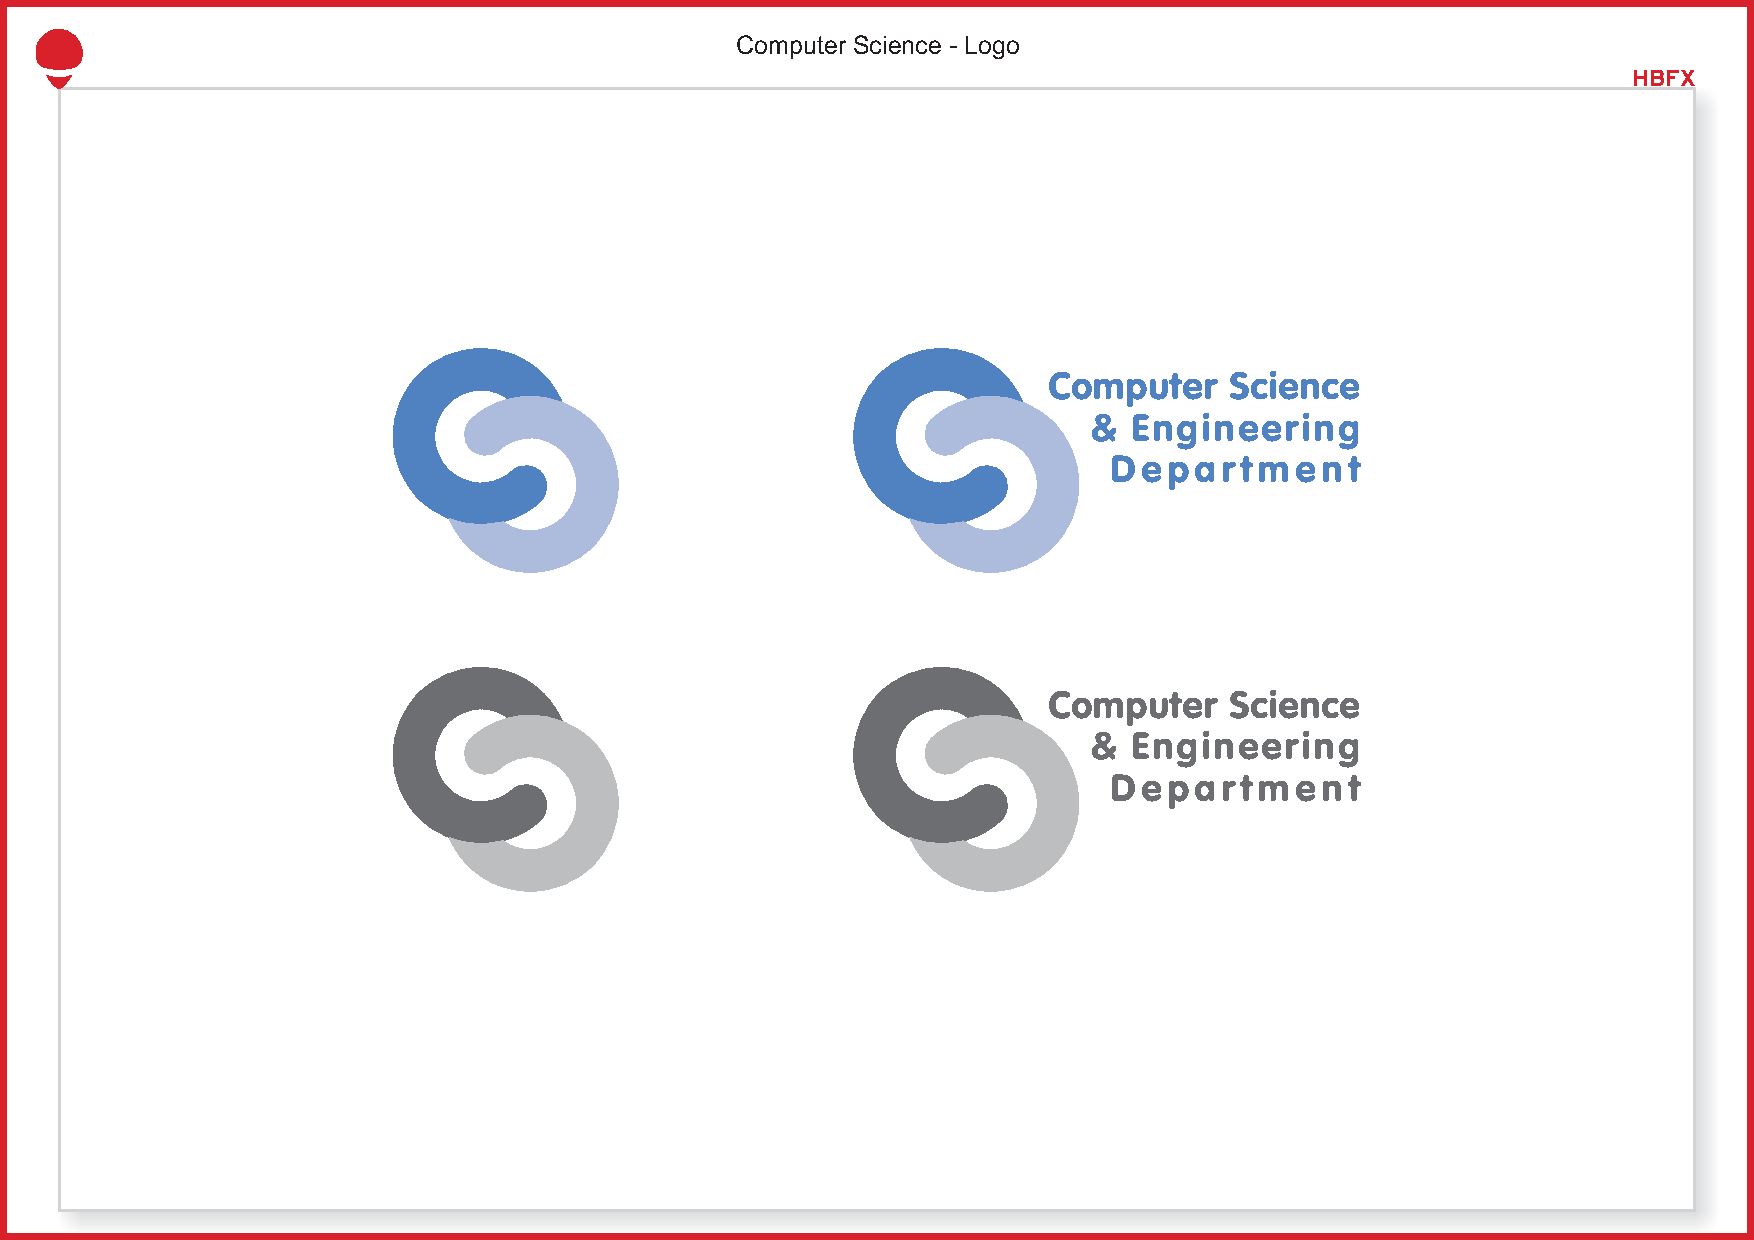
\includegraphics[scale=0.5,trim={14cm 11cm 2cm 5cm},clip=true]{pics/cs-logo.pdf}}%
  {\fbox{\parbox[c][2.8cm][c]{3.2cm}{\centering\small [pics/cs-logo.pdf]}}}
\end{tabular}

\vspace{105pt}
{\Huge #2}\\                           % diploma project text
\vspace{40pt}
{\Large #3}\\ \vspace{0pt}  % project title
{\Large #4}\\                          % project subtitle
\vspace{40pt}
{\LARGE \Name}\\                   % student name
\end{center}
\vspace{60pt}
\begin{tabular*}{\textwidth}{@{\extracolsep{\fill}}p{6cm}r}
&{\large\textbf{#5}}\vspace{10pt}\\      % scientific advisor
&{\large \Advisor}                                    % advisor name
\end{tabular*}
\vspace{20pt}
\begin{center}
{\large\textbf{#6}}\\                                % bucharest
\vspace{0pt}
{\normalsize \Year}
\end{center}
\end{titlepage}
}

\newcommand{\frontPageRO}{\frontPage{\UniTextRO}{\DiplomaRO}{\ProjectTitleRO}{\ProjectSubtitleRO}{\AdvisorRO}{\BucRO}}
\newcommand{\frontPageEN}{\frontPage{\UniTextEN}{\DiplomaEN}{\ProjectTitleEN}{\ProjectSubtitleEN}{\AdvisorEN}{\BucEN}}

\linespread{1.15}
\setlength\parindent{0pt}
\setlength\parskip{.28cm}

%% Abstract macro
\newcommand{\AbstractPage}{
\begin{titlepage}
\textbf{\large SINOPSIS}\par
\AbstractRO\par\vfill
\textbf{\large ABSTRACT}\par
\AbstractEN \vfill
\end{titlepage}
}

%% Thank you macro
\newcommand{\ThanksPage}{
\begin{titlepage}
{\noindent \large\textbf{MULȚUMIRI}}\\
\Thanks
\end{titlepage}
}

%%%%%%%%%%%%%%%%%%%%%%%%%%%%%%%%%%%%%%%%%%%%%%%%%%
%%
%%   Câmpurile de mai jos sunt completate de autor
%%
%%%%%%%%%%%%%%%%%%%%%%%%%%%%%%%%%%%%%%%%%%%%%%%%%%

\newcommand{\ProjectTitleRO}{RevBid --- Platformă web pentru licitații inverse}
\newcommand{\ProjectSubtitleRO}{Sistem informatic pentru achiziții B2B competitive}
\newcommand{\ProjectTitleEN}{RevBid --- A Web Platform for Reverse Auctions}
\newcommand{\ProjectSubtitleEN}{An Information System for Competitive B2B Procurement}
\newcommand{\Name}{Tudor Crețu}
% TODO: completează numele coordonatorului științific (ex: Prof. dr. ing. Andrei Ionescu)
\newcommand{\Advisor}{\todoinline{Titlu Prenume NUME --- coordonator}}
\newcommand{\Year}{2026}

% Setări document
\title{Proiect de diplomă}
\author{\Name}
\date{\Year}

%%
%%   Câmpurile aferente rezumatului
%%
\newcommand{\AbstractRO}{Lucrarea prezintă proiectarea, implementarea și evaluarea platformei RevBid, un sistem informatic web pentru licitații inverse destinat achizițiilor dintre companii (B2B). Spre deosebire de licitațiile clasice, în licitația inversă cumpărătorul publică o cerere de produse sau servicii, iar furnizorii concurează între ei prin oferte de preț din ce în ce mai mici, câștigând oferta cea mai avantajoasă la momentul închiderii. RevBid acoperă întregul ciclu de viață al unei astfel de achiziții: crearea cererii (inclusiv salvarea ca draft), ofertarea în timp real prin WebSocket --- cu tratarea corectă a ofertelor concurente și prelungirea automată a termenului împotriva practicii de tip „sniping'' ---, închiderea automată programată, notificări multi-canal (aplicație și email), generarea unui document PDF de rezumat al tranzacției, confirmarea bilaterală a livrării și primirii, recenzii reciproce și statistici agregate pentru ambele roluri. Soluția este construită ca aplicație single-page în React, cu un API REST în Node.js/Express, baza de date MongoDB și comunicare în timp real prin Socket.IO, integrând mecanisme de securitate precum autentificarea JWT în cookie httpOnly, controlul accesului pe roluri, limitarea ratei cererilor și jurnalizarea de audit. Evaluarea a urmărit corectitudinea funcțională pe scenarii end-to-end și măsurători de performanță, rezultatele confirmând viabilitatea platformei pentru întreprinderi mici și mijlocii.}

\newcommand{\AbstractEN}{This thesis presents the design, implementation and evaluation of RevBid, a web-based reverse auction system for business-to-business (B2B) procurement. Unlike classical auctions, in a reverse auction the buyer publishes a request for products or services and suppliers compete against each other by submitting increasingly lower price bids, with the most advantageous offer winning at closing time. RevBid covers the entire life cycle of such an acquisition: request creation (including draft saving), real-time bidding over WebSocket --- with correct handling of concurrent bids and automatic deadline extension against sniping ---, scheduled automatic closing, multi-channel notifications (in-app and email), generation of a PDF transaction summary document, bilateral delivery and receipt confirmation, mutual reviews and aggregated statistics for both roles. The solution is built as a single-page application in React, with a REST API in Node.js/Express, a MongoDB database and real-time communication through Socket.IO, integrating security mechanisms such as JWT authentication stored in an httpOnly cookie, role-based access control, request rate limiting and audit logging. The evaluation covered functional correctness on end-to-end scenarios and performance measurements, with results confirming the platform's viability for small and medium enterprises.}

%%
%%   Câmpurile aferente paginii de mulțumiri
%%
% TODO: personalizează sau comentează \ThanksPage din document dacă nu o folosești
\newcommand{\Thanks}{\todoinline{Opțional --- mulțumiri adresate coordonatorului, familiei, colegilor etc. Dacă nu dorești această pagină, comentează linia \texttt{\textbackslash ThanksPage} de mai jos.}}

\begin{document}

\frontPageRO
\frontPageEN

\begingroup
\linespread{1}
\tableofcontents
\endgroup

\AbstractPage

% poate fi comentată sau ștearsă
\ThanksPage


% Textul licenței începe de aici

\chapter{Introducere}\pagestyle{fancy}

Acest capitol introduce contextul în care se încadrează lucrarea, formulează problema abordată, prezintă obiectivele urmărite și oferă o privire de ansamblu asupra soluției propuse --- platforma \textbf{RevBid} --- precum și asupra rezultatelor obținute și a structurii lucrării.

\section{Context}

Digitalizarea proceselor de achiziție reprezintă una dintre direcțiile majore de transformare a mediului de afaceri, comerțul electronic dintre companii (\textit{business-to-business}, B2B) depășind ca volum, în mod constant, comerțul electronic către consumatorii finali, conform statisticilor europene privind comerțul electronic \cite{eurostatecom}. Încă de la finalul anilor '90, piețele electronice B2B (\textit{e-hubs}) au fost identificate drept un mecanism cu potențial ridicat de eficientizare a achizițiilor, tocmai pentru că agregă cererea și oferta și reduc costurile de tranzacționare, așa cum arată Kaplan și Sawhney \cite{kaplan2000}.

În acest peisaj, \textbf{licitația inversă} (\textit{reverse auction} sau \textit{procurement auction}) ocupă un loc special. Spre deosebire de licitația clasică (directă), în care vânzătorul oferă un bun iar cumpărătorii concurează prin prețuri din ce în ce mai mari, într-o licitație inversă rolurile sunt inversate: \textbf{cumpărătorul} publică o cerere pentru un produs sau serviciu (specificând cantitatea, termenul de livrare și, opțional, un preț țintă), iar \textbf{furnizorii} concurează între ei depunând oferte cu prețuri din ce în ce mai \textbf{mici}. La închiderea licitației câștigă furnizorul cu prețul cel mai avantajos. Fundamentele teoretice ale mecanismelor de licitație au fost puse de Vickrey \cite{vickrey1961} și sistematizate ulterior de McAfee și McMillan \cite{mcafee1987}, iar literatura dedicată licitațiilor inverse electronice documentează atât economiile de cost obținute de cumpărători, cât și condițiile în care acest instrument funcționează corect \cite{jap2002, smeltzer2003}.

Relevanța domeniului este confirmată și de practica industrială: suite enterprise precum SAP Ariba \cite{aribaweb} includ licitații inverse ca instrument standard de \textit{strategic sourcing}, iar în sectorul public românesc, Sistemul Electronic de Achiziții Publice (SEAP/SICAP) \cite{seapweb} folosește faze de re-ofertare electronică cu preț descrescător, în acord cu directivele europene privind achizițiile publice \cite{directive2014}.

\section{Problema}

Deși mecanismul licitației inverse este matur și validat, accesul la el este puternic polarizat. La un capăt se află soluțiile enterprise (SAP Ariba \cite{aribaweb}, Coupa \cite{coupaweb}), cu costuri de licențiere și implementare prohibitive pentru companiile mici; la celălalt capăt se află platformele publice de achiziții (SEAP/SICAP \cite{seapweb}), rezervate exclusiv contractelor cu autorități ale statului. Pentru \textbf{întreprinderile mici și mijlocii din mediul privat} nu există practic un instrument accesibil, în limba română, prin care o firmă să publice o cerere de achiziție și să obțină, transparent și în timp real, oferte competitive de la mai mulți furnizori.

În absența unui astfel de instrument, procesul tipic de achiziție al unui IMM rămâne manual: cereri de ofertă trimise individual prin email sau telefon, oferte primite în formate eterogene, imposibil de comparat direct, fără presiune concurențială reală între furnizori și fără trasabilitate. Acest mod de lucru ridică mai multe probleme concrete:

\begin{itemize}
    \item \textbf{lipsa concurenței transparente} --- furnizorii nu își văd reciproc ofertele, deci nu au motiv să își îmbunătățească prețul, iar literatura arată că tocmai dinamica competitivă vizibilă generează economiile \cite{jap2002, carter2004};
    \item \textbf{costuri de timp ridicate} --- colectarea și compararea manuală a ofertelor consumă zile sau săptămâni;
    \item \textbf{lipsa de încredere post-tranzacție} --- în afara unui cadru formal, nu există confirmări de livrare, documente de sinteză sau un istoric reputațional al partenerilor (recenzii), riscuri semnalate încă din primele studii asupra licitațiilor B2B online \cite{emiliani2000, smeltzer2003};
    \item \textbf{lipsa datelor decizionale} --- fără un sistem informatic, firmele nu pot măsura economiile obținute, categoriile cu cea mai bună competiție sau furnizorii cu care colaborează cel mai eficient.
\end{itemize}

Problema abordată de această lucrare este, prin urmare: \textit{proiectarea și implementarea unui sistem informatic complet pentru licitații inverse, accesibil IMM-urilor, care să acopere întregul ciclu de achiziție --- de la publicarea cererii și ofertarea competitivă în timp real, până la finalizarea tranzacției, documentele aferente și mecanismele de încredere reciprocă}.

\section{Obiective}

Obiectivul principal al proiectului este dezvoltarea unei platforme web funcționale de licitații inverse pentru achiziții B2B, denumită \textbf{RevBid}. Acesta se descompune în următoarele obiective specifice:

\begin{enumerate}
    \item \textbf{O1.} Implementarea ciclului de viață complet al unei licitații inverse: creare (inclusiv salvare ca \textit{draft}), publicare cu validare, ofertare descrescătoare, închidere automată la termen și desemnarea câștigătorului;
    \item \textbf{O2.} Ofertare \textbf{în timp real}: propagarea ofertelor și a prețului curent către toți participanții conectați, cu latență de ordinul sutelor de milisecunde, și tratarea corectă a ofertelor concurente (fără supra-scrieri sau stări inconsistente);
    \item \textbf{O3.} Descurajarea practicii de tip \textit{sniping} (oferte depuse în ultima secundă) prin prelungirea automată a termenului limită;
    \item \textbf{O4.} Construirea unui mecanism de \textbf{încredere} între părți: confirmarea bilaterală a livrării și primirii, recenzii reciproce cu rating agregat și un document PDF de rezumat al tranzacției generat automat;
    \item \textbf{O5.} Notificarea multi-canal a utilizatorilor (în aplicație, în timp real, și prin email) pentru toate evenimentele relevante;
    \item \textbf{O6.} Protejarea integrității licitațiilor active: modificarea sau ștergerea lor doar printr-un flux de aprobare supervizat de administrator, cu vizualizarea diferențelor;
    \item \textbf{O7.} Furnizarea de \textbf{statistici agregate} per rol (economii realizate, rată de câștig, categorii dominante etc.), calculate pe datele reale ale platformei;
    \item \textbf{O8.} Asigurarea unui nivel de securitate adecvat unei aplicații expuse public: autentificare robustă, control al accesului pe roluri, limitarea ratei cererilor și jurnalizare de audit.
\end{enumerate}

Atingerea acestor obiective oferă IMM-urilor un instrument care reduce costul achizițiilor prin competiție transparentă, comprimă durata procesului de la zile la ore și formalizează relația cumpărător--furnizor printr-un istoric verificabil.

\section{Soluția propusă}

Soluția propusă este \textbf{RevBid}, o platformă web de tip \textit{marketplace} cu trei roluri (cumpărător, furnizor, administrator), construită în jurul câtorva idei centrale.

În primul rând, licitația este modelată ca un proces cu stări explicite (draft $\to$ activă $\to$ închisă/anulată), în care regula fundamentală este \textbf{prețul strict descrescător}: fiecare ofertă nouă trebuie să fie mai mică decât prețul curent cu cel puțin un pas minim, iar câștigătorul este deținătorul ofertei minime la momentul închiderii. Ofertarea se desfășoară \textit{live}: toți participanții aflați pe pagina licitației văd instantaneu noile oferte, prețul curent și prelungirile de termen, ceea ce reproduce presiunea concurențială a unei licitații fizice.

În al doilea rând, corectitudinea competiției este tratată ca o problemă de proiectare, nu lăsată la voia întâmplării: ofertele concurente sunt arbitrate printr-o actualizare atomică de tip \textit{compare-and-set} la nivelul bazei de date (astfel încât din două oferte simultane doar una poate reuși), termenul limită se prelungește automat dacă o ofertă sosește în ultimele minute (anti-sniping), iar închiderea și notificarea finalizării sunt idempotente (nu pot fi executate de două ori, chiar la repornirea serverului).

În al treilea rând, platforma nu se oprește la desemnarea câștigătorului, ci formalizează și \textbf{etapa post-licitație}, acolo unde se construiește încrederea: sistemul generează automat un document de rezumat al tranzacției, cere confirmarea livrării de către furnizor și a primirii de către cumpărător și abia apoi deblochează recenziile reciproce, care alimentează rating-ul public al fiecărui utilizator. Modificările asupra licitațiilor active trec printr-un flux de aprobare administrat, cu evidențierea diferențelor între varianta veche și cea propusă, pentru ca ofertanții existenți să nu poată fi prejudiciați.

Din punct de vedere arhitectural, RevBid este o aplicație \textit{single-page} (React) care comunică cu un API REST (Node.js/Express) și primește evenimente în timp real printr-un canal WebSocket (Socket.IO), datele fiind stocate în MongoDB; detaliile și argumentele acestor alegeri sunt discutate în capitolele \ref{chap:piata} și \ref{chap:solutia}.

\section{Rezultatele obținute}

Rezultatul concret al proiectului este o platformă completă și funcțională, care implementează toate obiectivele enumerate: 14 modele de date, 13 module de rute REST, un canal de evenimente în timp real cu autentificare proprie, un job programat de închidere automată, generare de documente PDF cu numerotare secvențială, mesagerie privată și chat per licitație, centru de notificări cu livrare \textit{offline}, panou de administrare cu jurnal de audit și două dashboard-uri de statistici (cumpărător și furnizor) calculate prin agregări pe datele reale. Interfața --- 24 de pagini și 22 de componente reutilizabile React --- este integral în limba română.

Corectitudinea funcțională a fost verificată prin scenarii end-to-end pe un set de date de test reproductibil (20 de utilizatori, 55 de licitații, sute de oferte), incluzând scenarii de concurență cu oferte simultane din sesiuni diferite, iar performanța a fost evaluată prin măsurători de latență și de încărcare, prezentate în capitolul \ref{chap:evaluare}. Față de soluțiile existente analizate în capitolul \ref{chap:piata}, RevBid acoperă o nișă neadresată --- licitații inverse în timp real pentru mediul privat, cu flux post-tranzacție și mecanism de reputație integrate --- la un cost de operare apropiat de zero.

\section{Structura lucrării}

Restul lucrării este organizat după cum urmează. Capitolul \ref{chap:cerinte} analizează cerințele platformei pornind de la actorii implicați și scenariile de utilizare, rezultând lista cerințelor funcționale și non-funcționale. Capitolul \ref{chap:piata} trece în revistă fundamentele licitațiilor inverse din literatura de specialitate, analizează comparativ soluțiile existente pe piață și argumentează alegerile tehnologice față de alternativele lor. Capitolul \ref{chap:solutia} prezintă arhitectura soluției: structura generală client--server, modelul de date, ciclul de viață al licitației și fluxurile principale (ofertare în timp real, finalizare, post-licitație, aprobare a modificărilor). Capitolul \ref{chap:implementare} detaliază implementarea, cu accent pe punctele dificile din punct de vedere tehnic: arbitrarea ofertelor concurente, idempotența finalizării, autentificarea canalului WebSocket, generarea PDF cu diacritice și securitatea aplicației. Capitolul \ref{chap:evaluare} evaluează platforma pe două direcții --- corectitudine funcțională față de cerințe și performanță măsurată --- și o compară cu soluțiile existente. Capitolul \ref{chap:concluzii} sintetizează concluziile și direcțiile de dezvoltare ulterioară.

\chapter{Analiza cerințelor}
\label{chap:cerinte}

Acest capitol analizează cerințele platformei din perspectiva utilizatorilor vizați și a scenariilor de utilizare preconizate. Pornind de la motivația proiectului și de la actorii identificați, sunt derivate cerințele funcționale și non-funcționale care au ghidat proiectarea și pe baza cărora este evaluată soluția în capitolul \ref{chap:evaluare}.

\section{Motivație și public țintă}

Publicul țintă al platformei îl reprezintă \textbf{întreprinderile mici și mijlocii din mediul privat}, în dublă calitate: de \textit{cumpărători} (firme care achiziționează periodic produse sau servicii: echipamente IT, consumabile, materiale de construcții, servicii de transport, catering, mentenanță etc.) și de \textit{furnizori} (firme care vând astfel de produse/servicii și caută clienți noi fără costuri mari de vânzare).

Literatura de specialitate documentează consecvent faptul că licitațiile inverse electronice produc economii de preț semnificative pentru cumpărători și lărgesc baza de furnizori, cu condiția ca produsul să fie specificabil clar și competiția să fie reală \cite{jap2002, smeltzer2003, carter2004}. În același timp, studiile atrag atenția asupra riscurilor --- presiunea exclusivă pe preț poate afecta calitatea și relația cumpărător--furnizor \cite{emiliani2000, jap2002} --- ceea ce motivează direct două decizii de proiectare ale RevBid: descrierea detaliată și imuabilă a cererii (modificările asupra licitațiilor active necesită aprobare) și mecanismul de reputație bazat pe recenzii reciproce, care contrabalansează criteriul prețului.

\todoinline{Opțional, pentru întărirea acestei secțiuni: 1--2 paragrafe despre validarea cerințelor cu potențiali utilizatori reali --- de exemplu discuții/interviuri cu firme cunoscute (ce proces de achiziție au acum, ce le lipsește), sau feedback primit de la colegi/cunoscuți care au testat platforma. Menționează numărul de persoane, rolul lor și 2--3 concluzii care au influențat cerințele.}

Proiectul este realizat integral de autor (frontend, backend, baza de date, integrările externe), nefiind parte a unui proiect mai amplu împărțit între mai mulți studenți.

\section{Actori și scenarii de utilizare}

Platforma definește trei actori, cu responsabilități distincte:

\begin{itemize}
    \item \textbf{Cumpărătorul (buyer)} --- creează licitații (le poate salva ca draft), urmărește ofertele primite în timp real, comunică cu ofertanții prin chat-ul licitației, primește documentul de finalizare, confirmă primirea produselor/serviciilor și lasă recenzii furnizorilor;
    \item \textbf{Furnizorul (supplier)} --- explorează licitațiile active (cu filtre și căutare), depune oferte descrescătoare, este notificat când este supralicitat, confirmă livrarea în caz de câștig, lasă recenzii cumpărătorilor și își urmărește performanța în statistici;
    \item \textbf{Administratorul (admin)} --- supervizează platforma: gestionează utilizatorii (inclusiv suspendarea conturilor), arbitrează cererile de editare/ștergere a licitațiilor active și are vizibilitate asupra jurnalului de audit.
\end{itemize}

Scenariul de utilizare central al platformei (``firul roșu'' al întregului sistem) este următorul:

\begin{enumerate}
    \item Cumpărătorul își creează cont (email + parolă cu verificare prin cod, sau cont Google), își completează datele de companie și publică o cerere: \textit{„300 de scaune de birou ergonomice, livrare în 30 de zile, buget de pornire 45\,000 RON, preț țintă 30\,000 RON''}, cu termen limită peste 7 zile și prelungire automată activată;
    \item Furnizorii înregistrați văd licitația în lista celor active, se pot abona la ea și depun oferte; fiecare ofertă trebuie să fie mai mică decât prețul curent cu cel puțin pasul minim; toți cei conectați văd în timp real noua ofertă, prețul curent și graficul de evoluție;
    \item Un furnizor supralicitat primește instant notificare în aplicație și email și poate reveni cu o ofertă mai bună; ofertele din ultimele 2 minute prelungesc automat termenul cu 5 minute;
    \item La atingerea termenului, sistemul închide automat licitația, desemnează câștigătorul (oferta minimă), generează documentul PDF „Rezumat de tranzacție'' și notifică toate părțile (câștigător, cumpărător, ofertanți necâștigători, abonați);
    \item Furnizorul livrează și confirmă livrarea în platformă; cumpărătorul confirmă primirea; ambele confirmări deblochează recenziile reciproce (1--5 stele), care actualizează rating-ul public al fiecăruia;
    \item Ambii își consultă statisticile: cumpărătorul vede economiile realizate față de buget, furnizorul își vede rata de câștig și licitațiile pierdute la limită.
\end{enumerate}

Figura~\ref{fig:diagrama-cazuri-utilizare} sintetizează cazurile de utilizare pe actori.

% ── FIGURĂ DE CREAT: diagramă de cazuri de utilizare (draw.io / PlantUML) ──
% Sugestie de conținut: 3 actori (Cumpărător, Furnizor, Administrator) și
% cazurile majore: creare/publicare licitație, salvare draft, ofertare,
% abonare, chat licitație, mesagerie, confirmare livrare/primire, recenzie,
% cerere editare/ștergere, aprobare cereri, gestionare utilizatori, statistici.
\placeholderfig{0.95}{diagrama-cazuri-utilizare}{8.5cm}{Diagramă UML de cazuri de utilizare cu cei 3 actori (Cumpărător, Furnizor, Administrator) și cazurile de utilizare principale ale fiecăruia. Se poate realiza în draw.io sau PlantUML.}{Diagrama cazurilor de utilizare ale platformei RevBid}

\section{Cerințe funcționale}

Din scenariile de mai sus a fost derivată lista cerințelor funcționale, grupate pe module și sumarizate în Tabelul~\ref{tab:cerinte-functionale}. Prioritatea folosește notația MoSCoW simplificată: \textbf{M} (must have --- esențială), \textbf{S} (should have --- importantă), \textbf{C} (could have --- opțională).

\begin{table}[!ht]\small\linespread{1}
\centering
\caption{Cerințele funcționale ale platformei RevBid}
\label{tab:cerinte-functionale}
\begin{tabular}{l >{\raggedright\arraybackslash}p{11.2cm} c}
\toprule
\textbf{ID} & \textbf{Cerință} & \textbf{Prio.} \\
\midrule
\multicolumn{3}{l}{\textit{Conturi și autentificare}} \\
RF-01 & Înregistrare cu email și parolă, alegerea rolului (cumpărător/furnizor) și activarea contului printr-un cod de verificare trimis pe email & M \\
RF-02 & Autentificare alternativă cu cont Google (OAuth 2.0) & S \\
RF-03 & Resetarea parolei printr-un link trimis pe email, cu valabilitate limitată & M \\
RF-04 & Gestionarea profilului și a datelor de companie/fiscale (denumire legală, CUI/CIF, Registrul Comerțului, sediu social), folosite în documentele generate & M \\
\midrule
\multicolumn{3}{l}{\textit{Gestiunea licitațiilor}} \\
RF-05 & Crearea unei licitații cu titlu, descriere, categorie, cantitate, buget de pornire, preț țintă (opțional), termen limită, imagini, locație pe hartă și etichete & M \\
RF-06 & Salvarea licitației ca \textit{draft} (incomplet) și publicarea ulterioară, cu validarea completă a câmpurilor obligatorii doar la publicare & M \\
RF-07 & Listarea, căutarea și filtrarea licitațiilor (categorie, status, text); drafturile sunt vizibile exclusiv proprietarului & M \\
RF-08 & Editarea/ștergerea licitațiilor: directă pentru drafturi; pentru licitațiile active, doar prin cerere aprobată de administrator, cu vizualizarea diferențelor vechi/nou & M \\
\midrule
\multicolumn{3}{l}{\textit{Ofertare}} \\
RF-09 & Depunerea de oferte de către furnizori, cu preț strict descrescător (cu cel puțin pasul minim sub prețul curent) și mesaj opțional & M \\
RF-10 & Propagarea în timp real a ofertelor, a prețului curent și a istoricului către toți utilizatorii aflați pe pagina licitației & M \\
RF-11 & Prelungirea automată a termenului limită când o ofertă sosește în ultimele minute (anti-sniping), configurabilă per licitație & S \\
RF-12 & Istoric complet al ofertelor și grafic de evoluție a prețului & S \\
\midrule
\multicolumn{3}{l}{\textit{Finalizare și post-licitație}} \\
RF-13 & Închiderea automată a licitațiilor la termen și desemnarea câștigătorului (oferta cu valoarea minimă) & M \\
RF-14 & Generarea automată a unui document PDF „Rezumat de tranzacție'', cu numerotare secvențială și datele fiscale ale părților & S \\
RF-15 & Confirmarea livrării de către furnizor și a primirii de către cumpărător & M \\
RF-16 & Recenzii reciproce (1--5 stele + comentariu), deblocate doar după dubla confirmare; rating agregat afișat pe profilul public & M \\
\midrule
\multicolumn{3}{l}{\textit{Comunicare și notificări}} \\
RF-17 & Notificări în aplicație, livrate în timp real, cu centru de notificări dedicat (paginare, filtre pe categorii, căutare, marcare citit/necitit) & M \\
RF-18 & Notificări email tranzacționale (ofertă nouă, supralicitare, finalizare, confirmări, resetare parolă, termen aproape de expirare) & S \\
RF-19 & Mesagerie privată între utilizatori (cu suport pentru imagini) și chat dedicat pe pagina fiecărei licitații (cumpărător + ofertanți) & S \\
RF-20 & Abonarea la licitații pentru a primi notificări despre evoluția lor & S \\
\midrule
\multicolumn{3}{l}{\textit{Administrare și analiză}} \\
RF-21 & Panou de administrare: gestionarea utilizatorilor (inclusiv suspendare), vizibilitate globală asupra licitațiilor, arbitrarea cererilor de editare/ștergere, jurnal de audit & M \\
RF-22 & Statistici agregate per rol: pentru cumpărător (economii totale și procentuale, buget publicat, categorii dominante, furnizori frecvenți, trend al economiilor), pentru furnizor (rată de câștig, valoare câștigată, distribuția ofertelor, licitații pierdute la limită, distribuția rating-ului) & S \\
\bottomrule
\end{tabular}
\end{table}

\section{Cerințe non-funcționale}

Cerințele non-funcționale, sumarizate în Tabelul~\ref{tab:cerinte-nefunctionale}, decurg din natura aplicației: o platformă tranzacțională expusă public, cu actualizări în timp real și date cu caracter comercial. Pragurile de performanță sunt formulate ca ținte verificabile, reluate la evaluare (capitolul \ref{chap:evaluare}); recomandările OWASP pentru aplicații web \cite{owasp2021} au fost folosite ca referință pentru cerințele de securitate.

\begin{table}[!ht]\small\linespread{1}
\centering
\caption{Cerințele non-funcționale ale platformei RevBid}
\label{tab:cerinte-nefunctionale}
\begin{tabular}{l >{\raggedright\arraybackslash}p{4cm} >{\raggedright\arraybackslash}p{9cm}}
\toprule
\textbf{ID} & \textbf{Categorie} & \textbf{Cerință} \\
\midrule
RNF-01 & Securitate --- autentificare & Parole stocate exclusiv ca hash (bcrypt); politică de complexitate la înregistrare; token de sesiune semnat (JWT), păstrat în cookie httpOnly, inaccesibil din JavaScript \\
RNF-02 & Securitate --- autorizare & Control al accesului pe roluri și pe proprietate (un utilizator nu poate modifica resursele altuia); drafturile sunt invizibile pentru terți \\
RNF-03 & Securitate --- abuz & Limitarea ratei cererilor pe operațiunile sensibile (autentificare, creare licitație, mesaje, recenzii, upload) și suspendarea conturilor abuzive, inclusiv pe canalul în timp real \\
RNF-04 & Corectitudine & Arbitrarea deterministă a ofertelor concurente (două oferte simultane nu pot fi ambele acceptate); operațiunile de finalizare sunt idempotente (re-execuția nu duplică efectele) \\
RNF-05 & Performanță & Propagarea unei oferte către participanți în sub 1 secundă în condiții normale; răspunsuri API sub 200 ms (mediană) pentru operațiunile de listare pe setul de date de test \\
RNF-06 & Utilizabilitate & Interfață integral în limba română, cu diacritice corecte (inclusiv în emailuri și PDF-uri); design responsive, utilizabil pe desktop și mobil \\
RNF-07 & Confidențialitate & Datele sensibile (emailuri, identificatori fiscali) sunt mascate în jurnale; secretele aplicației provin exclusiv din variabile de mediu \\
RNF-08 & Mentenabilitate & Cod organizat modular (modele/rute/servicii/middleware); jurnalizare structurată cu identificator de cerere și niveluri distincte (audit, securitate, eroare) \\
RNF-09 & Scalabilitate & Interogări susținute de indexuri adecvate; liste paginate; agregările statistice nu blochează operațiunile curente \\
RNF-10 & Compatibilitate & Funcționare în browserele moderne (Chrome, Firefox, Edge), fără plugin-uri \\
\bottomrule
\end{tabular}
\end{table}

\section{Procesul de elaborare a cerințelor}

Cerințele nu au fost fixate integral la început, ci au evoluat \textbf{iterativ}, pe modelul MVP (\textit{minimum viable product}) urmat de reevaluări succesive. Prima iterație a acoperit nucleul funcțional (conturi, licitații, ofertare în timp real, dashboard-uri); pe baza utilizării efective a acestui MVP au fost identificate lipsuri care au generat iterațiile următoare, reflectate și în istoricul de versiuni al proiectului: sistemul de drafturi și pagina dedicată de notificări (publicarea „totul sau nimic'' s-a dovedit nepractică pentru cereri complexe), fluxul post-licitație cu documente, confirmări și recenzii (cerință de încredere semnalată la testare), datele de companie/fiscale (necesare pentru ca documentele generate să aibă valoare practică), diacriticele complete în întreaga platformă și, în final, statisticile agregate pe roluri.

\todoinline{Dacă ai obținut feedback de la utilizatori reali între iterații (colegi, cunoscuți cu firme, coordonator), descrie aici concret: cine a testat, ce a semnalat și ce cerințe au rezultat. Întărește criteriul de proces iterativ cu utilizatori.}

\chapter{Studiu de piață și tehnologii}
\label{chap:piata}

Acest capitol poziționează lucrarea în contextul existent, pe trei planuri: fundamentele licitațiilor inverse din literatura de specialitate, soluțiile comerciale și publice disponibile pe piață (cu limitările lor) și tehnologiile alese pentru implementare, analizate comparativ cu alternativele relevante.

\section{Licitațiile inverse în literatura de specialitate}

Teoria licitațiilor distinge patru formate clasice: licitația engleză (ascendentă, deschisă), licitația olandeză (descendentă, deschisă), licitația cu ofertă sigilată de prim preț și licitația Vickrey (ofertă sigilată, al doilea preț), ale cărei proprietăți de stimulare a ofertării oneste au fost demonstrate de Vickrey \cite{vickrey1961}. McAfee și McMillan \cite{mcafee1987} definesc licitația drept „o instituție de piață cu un set explicit de reguli care determină alocarea resurselor și prețurile pe baza ofertelor participanților'' și analizează echivalențele de venit dintre formate, iar Klemperer \cite{klemperer1999} oferă o sistematizare a întregii literaturi.

\textbf{Licitația inversă} (numită și licitație de achiziție --- \textit{procurement auction}) inversează rolurile: un singur cumpărător, mai mulți vânzători concurenți, preț descrescător. Formatul implementat de RevBid este echivalentul invers al licitației engleze: licitație \textit{deschisă}, în care participanții văd prețul curent și pot reveni cu oferte îmbunătățite până la termenul limită. Formal, dacă $B = \{b_1, b_2, \ldots, b_n\}$ este mulțimea ofertelor valide depuse până la închidere, câștigătorul $w$ este:

\begin{equation}
\label{eq:castigator}
w = \arg\min_{i \in \{1,\ldots,n\}} b_i
\end{equation}

Literatura empirică asupra licitațiilor inverse \textit{electronice} (B2B) s-a dezvoltat odată cu piețele online de la începutul anilor 2000. Kaplan și Sawhney \cite{kaplan2000} încadrează licitațiile inverse în taxonomia piețelor electronice B2B (\textit{e-hubs}), ca mecanism de agregare dinamică a prețului. Jap \cite{jap2002} analizează dinamica ofertării și efectele asupra relației cumpărător--furnizor, arătând că formatul deschis intensifică competiția, dar poate eroda încrederea furnizorilor dacă procesul nu este transparent și corect administrat. Smeltzer și Carr \cite{smeltzer2003} identifică condițiile de succes --- specificații clare ale produsului, număr suficient de furnizori calificați, volum atractiv --- și riscurile percepute de ambele părți. Emiliani \cite{emiliani2000} documentează problemele practice ale primelor implementări B2B (calitate, costuri ascunse, comportament oportunist), iar Carter et al. \cite{carter2004}, printr-un studiu calitativ pe cumpărători și furnizori, arată că economiile de preț trebuie puse în balanță cu costurile relaționale.

Din această literatură rezultă direct câteva decizii de proiectare ale RevBid: (i) formatul deschis cu preț curent vizibil (maximizează competiția \cite{jap2002}); (ii) pasul minim de scădere a ofertei, care previne „zgomotul'' ofertelor simbolice; (iii) prelungirea automată a termenului, care elimină avantajul ofertelor de ultimă secundă și apropie rezultatul de echilibrul teoretic al licitației engleze \cite{mcafee1987}; (iv) mecanismul de reputație (recenzii reciproce) și fluxul formal post-licitație, care adresează exact deficitul de încredere semnalat de \cite{emiliani2000, smeltzer2003}.

\section{Soluții existente pe piață}

\subsection{Platforme enterprise: SAP Ariba și Coupa}

SAP Ariba \cite{aribaweb} este liderul pieței de \textit{strategic sourcing}: include evenimente de tip RFI/RFP și licitații inverse în timp real, management de contracte și o rețea globală de furnizori. Coupa \cite{coupaweb} oferă o suită similară de \textit{business spend management}. Ambele sunt orientate exclusiv către corporații: implementarea presupune proiecte de integrare de luni de zile, licențierea se negociază la nivel de companie (costuri anuale de ordinul zecilor de mii de euro), iar interfețele --- nelocalizate în română --- presupun echipe dedicate de achiziții. Pentru un IMM care organizează câteva achiziții pe lună, raportul cost/beneficiu este prohibitiv.

\subsection{Sectorul public: SEAP/SICAP}

Sistemul Electronic de Achiziții Publice \cite{seapweb} este platforma națională prin care autoritățile contractante din România derulează achiziții publice, în conformitate cu directivele europene \cite{directive2014}. SEAP include „licitația electronică'' ca fază finală de re-ofertare cu preț descrescător --- conceptual identică licitației inverse. Limitările sunt însă structurale: platforma este rezervată \textbf{exclusiv} sectorului public (firmele private nu pot publica cereri proprii), procedurile sunt formalizate prin lege (documentații, garanții, termene rigide), iar experiența de utilizare este orientată spre conformitate, nu spre dinamica licitației (fără actualizări live, fără mecanisme de reputație între părți).

\subsection{Piețe globale de sourcing: Alibaba RFQ}

Serviciul RFQ (\textit{Request for Quotation}) al platformei Alibaba \cite{alibabarfq} permite cumpărătorilor să publice cereri la care furnizorii răspund cu cotații. Modelul este însă de tip „cereri--cotații'': ofertele sunt private, fără competiție vizibilă în timp real și fără preț curent care să scadă, deci fără presiunea concurențială specifică licitației inverse. Platforma este globală (orientată spre import din Asia), nelocalizată pentru piața românească, iar fluxul post-tranzacție (livrare, încredere) este gestionat în afara cererii propriu-zise.

\subsection{Platforme de servicii cu ofertare: Freelancer}

Platformele de tip Freelancer \cite{freelancerweb} aplică un mecanism înrudit pentru servicii digitale: clientul publică un proiect, prestatorii depun oferte, de regulă vizibile, iar clientul alege manual câștigătorul. Diferențele față de o licitație inversă reală sunt importante: prețul nu este forțat să scadă (ofertele nu se raportează la un preț curent), nu există termen cu închidere automată și desemnare deterministă a câștigătorului, iar domeniul este limitat la servicii pentru consumatori și micro-afaceri, nu achiziții B2B de produse.

\subsection{Sinteză comparativă și oportunitate}

Tabelul~\ref{tab:comparatie-piata} sintetizează comparația pe criteriile relevante pentru publicul țintă definit în capitolul \ref{chap:cerinte}.

\begin{table}[!ht]\footnotesize\linespread{1}
\centering
\caption{Comparația soluțiilor existente cu platforma propusă}
\label{tab:comparatie-piata}
\begin{tabular}{>{\raggedright\arraybackslash}p{3.6cm} c c c c c}
\toprule
\textbf{Criteriu} & \textbf{Ariba/Coupa} & \textbf{SEAP} & \textbf{Alibaba RFQ} & \textbf{Freelancer} & \textbf{RevBid} \\
\midrule
Licitație inversă cu preț descrescător & Da & Da (faza finală) & Nu & Parțial & Da \\
Ofertare în timp real (live) & Da & Nu & Nu & Nu & Da \\
Accesibil IMM-urilor private & Nu & Nu & Da & Da & Da \\
Cost pentru o firmă mică & Foarte ridicat & --- & Scăzut & Comision & Zero \\
Localizare română & Nu & Da & Nu & Nu & Da \\
Anti-sniping (prelungire automată) & Da & Nu & --- & Nu & Da \\
Flux post-licitație (livrare/primire) & Da & Parțial & Nu & Parțial & Da \\
Recenzii reciproce / reputație & Parțial & Nu & Parțial & Da & Da \\
Document de tranzacție generat & Da & Da & Nu & Nu & Da \\
Statistici pentru utilizator & Da & Nu & Nu & Parțial & Da \\
\bottomrule
\end{tabular}
\end{table}

Concluzia analizei: există un \textbf{gol clar de piață} între platformele enterprise (complete, dar inaccesibile IMM-urilor) și platformele deschise (accesibile, dar fără licitație inversă reală în timp real și fără flux post-tranzacție). RevBid țintește exact această nișă: licitații inverse \textit{live}, în limba română, gratuite, cu mecanisme integrate de încredere.

\section{Tehnologii utilizate și alternative}

Această secțiune prezintă stack-ul tehnologic ales și argumentează fiecare alegere față de alternativele uzuale. Criteriile de selecție au fost: potrivirea cu cerințele (în special timpul real --- RNF-05 și RF-10), productivitatea unui singur dezvoltator, maturitatea ecosistemului și costul de operare zero.

\subsection{Limbajul și platforma serverului: Node.js}

Backend-ul folosește \textbf{Node.js} cu framework-ul \textbf{Express 5} \cite{expressdocs}. Modelul de execuție al Node.js --- o buclă de evenimente cu I/O non-blocant --- este potrivit în mod natural pentru aplicații cu multe conexiuni concurente de tip notificare/difuzare, așa cum arată Tilkov și Vinoski \cite{tilkov2010}: serverul petrece majoritatea timpului așteptând I/O (bază de date, email), nu calculând, deci un singur fir de execuție poate servi mii de conexiuni WebSocket simultane. Alternativele luate în calcul:

\begin{itemize}
    \item \textbf{Spring Boot (Java)} --- matur, puternic tipizat, dar cu un cost de dezvoltare sensibil mai mare pentru un proiect individual și un model bazat pe fire de execuție mai costisitor pentru mii de conexiuni persistente;
    \item \textbf{Django (Python)} --- foarte productiv pentru CRUD, însă suportul WebSocket necesită componente suplimentare (Channels, server ASGI separat), complicând arhitectura;
    \item \textbf{NestJS (Node.js)} --- ar fi adus structură suplimentară (module, injecție de dependențe), dar cu un strat de abstractizare nejustificat la dimensiunea actuală a proiectului.
\end{itemize}

Argumentul decisiv pentru Node.js/Express a fost \textbf{unificarea limbajului}: JavaScript pe client și pe server elimină comutarea de context, permite partajarea convențiilor de validare și face ca integrarea Socket.IO (bibliotecă nativă Node.js) să fie directă.

\subsection{Stocarea datelor: MongoDB}

Persistența folosește \textbf{MongoDB} \cite{mongodocs}, o bază de date orientată pe documente \cite{chodorow2013}, accesată prin ODM-ul \textbf{Mongoose} \cite{mongoosedocs}, care adaugă scheme, validări și indexuri declarative. Alegerea față de o bază relațională (PostgreSQL/MySQL) se sprijină pe trei caracteristici ale domeniului:

\begin{itemize}
    \item \textbf{drafturile} --- o licitație draft poate avea orice subset de câmpuri completate; modelul pe documente permite acest lucru natural, validarea strictă fiind aplicată la nivel de aplicație doar la publicare (în relațional ar fi necesare coloane nullable peste tot sau tabele separate draft/activ);
    \item \textbf{sub-documentele și instantaneele} --- datele de companie sunt înglobate în documentul utilizatorului (relație 1:1, fără join-uri), iar documentul de tranzacție copiază un \textit{snapshot} al datelor la momentul finalizării, rămânând stabil chiar dacă profilurile se schimbă ulterior --- un șablon firesc pe documente;
    \item \textbf{operațiile atomice pe document} --- arbitrarea ofertelor concurente folosește actualizări condiționate atomice de tip \textit{compare-and-set} pe documentul licitației (detaliat în capitolul \ref{chap:implementare}), suficiente pentru consistența necesară fără tranzacții distribuite.
\end{itemize}

Compromisul acceptat: lipsa join-urilor native și a constrângerilor referențiale impune disciplina referințelor în aplicație (Mongoose \texttt{populate}) și agregări explicite pentru rapoarte --- acceptabil pentru schema relativ simplă a domeniului (14 colecții).

\subsection{Comunicarea în timp real: WebSocket și Socket.IO}

Cerința RF-10 (propagare live a ofertelor) impune un canal de comunicare de la server către client. Tabelul~\ref{tab:comparatie-realtime} compară mecanismele uzuale.

\begin{table}[!ht]\small\linespread{1}
\centering
\caption{Mecanisme de actualizare în timp real --- comparație}
\label{tab:comparatie-realtime}
\begin{tabular}{>{\raggedright\arraybackslash}p{3.4cm} >{\raggedright\arraybackslash}p{3.4cm} >{\raggedright\arraybackslash}p{3.4cm} >{\raggedright\arraybackslash}p{3.6cm}}
\toprule
\textbf{Mecanism} & \textbf{Latență} & \textbf{Cost server} & \textbf{Observații} \\
\midrule
Polling periodic & Egală cu intervalul de interogare (secunde) & Ridicat --- cereri repetate inutile & Simplu, dar irosește resurse și nu este „live'' \\
Long-polling & Sub-secundă & Mediu --- reconectări repetate & Compatibilitate bună, complexitate pe server \\
Server-Sent Events & Sub-secundă & Scăzut & Doar server$\to$client; insuficient pentru depunerea ofertelor pe același canal \\
WebSocket \cite{rfc6455} & Zeci de milisecunde & Scăzut --- o conexiune persistentă & Bidirecțional, full-duplex; alegerea naturală \\
\bottomrule
\end{tabular}
\end{table}

Protocolul WebSocket \cite{rfc6455} oferă o conexiune persistentă, bidirecțională, cu overhead minim per mesaj --- exact profilul necesar ofertării (clientul trimite oferta, serverul difuzează rezultatul tuturor). Peste WebSocket, a fost aleasă biblioteca \textbf{Socket.IO} \cite{socketiodocs}, care adaugă: (i) \textit{camere} (rooms) --- difuzare țintită către participanții unei licitații sau către sesiunile unui utilizator; (ii) \textit{callback-uri de confirmare} (acknowledgements) --- emitentul ofertei primește sincron succes/eroare; (iii) reconectare automată cu fallback pe long-polling; (iv) middleware de autentificare pe handshake. Implementarea manuală a acestor mecanisme peste WebSocket „pur'' (biblioteca \texttt{ws}) ar fi reinventat exact aceste componente.

\subsection{Interfața client: React și ecosistemul său}

Frontend-ul este o aplicație \textit{single-page} \cite{mikowski2013} construită cu \textbf{React 19} \cite{reactdocs}. Tabelul~\ref{tab:comparatie-frontend} rezumă comparația cu alternativele majore.

\begin{table}[!ht]\small\linespread{1}
\centering
\caption{Framework-uri de interfață --- comparație calitativă}
\label{tab:comparatie-frontend}
\begin{tabular}{>{\raggedright\arraybackslash}p{2.4cm} >{\raggedright\arraybackslash}p{3.6cm} >{\raggedright\arraybackslash}p{3.4cm} >{\raggedright\arraybackslash}p{4.2cm}}
\toprule
\textbf{Framework} & \textbf{Model} & \textbf{Curbă de învățare} & \textbf{Ecosistem} \\
\midrule
React \cite{reactdocs} & Bibliotecă de componente, stare unidirecțională & Medie & Cel mai larg (biblioteci pentru rutare, grafice, hărți etc.) \\
Angular & Framework complet, TypeScript obligatoriu & Abruptă & Larg, orientat enterprise \\
Vue & Framework progresiv & Lină & Larg, dominant în Asia \\
Svelte & Compilator (fără virtual DOM) & Lină & În creștere, mai restrâns \\
\bottomrule
\end{tabular}
\end{table}

Pentru natura aplicației --- pagini cu stare bogată, actualizate frecvent de evenimente externe (oferte sosite pe socket) --- modelul declarativ al React (starea determină interfața, re-randare la schimbarea stării) se potrivește direct: o ofertă nouă actualizează starea, iar prețul, lista de oferte și graficul se actualizează consistent. Dimensiunea ecosistemului, vizibilă în sondaje precum State of JS \cite{stateofjs} și în statisticile de descărcări npm \cite{npmtrends}, a cântărit de asemenea: toate bibliotecile auxiliare necesare au integrare React de primă clasă --- \textbf{React Router 7} pentru rutare client, \textbf{Chart.js} \cite{chartjsdocs} (prin \texttt{react-chartjs-2}) pentru graficele de evoluție a prețului și statistici, \textbf{Leaflet} \cite{leafletdocs} (prin \texttt{react-leaflet}) pentru hărți.

Figura~\ref{fig:npm-trends} ilustrează cantitativ dominanța ecosistemului React în perioada dezvoltării proiectului.

% ── FIGURĂ DE CREAT: captură de pe npmtrends.com ──
% Sugestie: intră pe npmtrends.com, compară react vs vue vs @angular/core vs svelte
% (interval 5 ani), fă captură graficului de descărcări săptămânale.
\placeholderfig{0.9}{npm-trends}{6.5cm}{Captură de ecran de pe npmtrends.com cu descărcările săptămânale npm pentru react, vue, @angular/core și svelte (ultimii 5 ani). Sursa se citează în notă de subsol.}{Popularitatea framework-urilor de interfață --- descărcări săptămânale npm \protect\cite{npmtrends}}

Pentru hărți, alternativa Google Maps API a fost respinsă din motive de cost și licențiere (cheie API cu facturare); Leaflet cu hărți OpenStreetMap este gratuit și suficient funcțional pentru selectarea și afișarea locației de livrare. Pentru grafice, Chart.js a fost preferat lui D3.js (nivel de abstractizare mult mai potrivit --- D3 ar fi însemnat construirea manuală a fiecărui element grafic) și lui Recharts (Chart.js este independent de framework și mai performant pe seturi mari de puncte, prin randare pe canvas).

Ca unealtă de build a fost folosit \textbf{Vite} \cite{vitedocs}, care oferă pornire instantanee a serverului de dezvoltare și \textit{hot module replacement} prin module ES native, față de bundler-ele clasice bazate pe webpack (de exemplu Create React App, între timp abandonat oficial) la care fiecare pornire recompilează întreaga aplicație. În dezvoltare, diferența este resimțită la fiecare salvare de fișier; o cuantificare pe proiectul de față este inclusă în capitolul \ref{chap:evaluare}.

\subsection{Autentificare și securitate}

Sesiunile API folosesc \textbf{JSON Web Tokens} \cite{rfc7519}: serverul emite la autentificare un token semnat (HMAC) conținând identitatea și rolul utilizatorului, verificabil ulterior fără stare pe server --- esențial pentru că același token autentifică atât cererile REST, cât și handshake-ul Socket.IO. Alternativa sesiunilor stocate pe server ar fi cerut un mecanism separat pentru WebSocket și stocare partajată la scalare. Compromisul JWT (imposibilitatea revocării imediate) este atenuat prin durata limitată (7 zile) și prin verificări suplimentare în baza de date la conexiunile socket (detaliat în capitolul \ref{chap:implementare}). Tokenul este transportat într-un cookie \texttt{httpOnly} --- inaccesibil scripturilor, deci protejat de furt prin XSS --- conform recomandărilor OWASP \cite{owasp2021}.

Parolele sunt protejate cu \textbf{bcrypt} \cite{provos1999}, o funcție de derivare costisitoare computațional și adaptabilă (factor de cost configurabil), proiectată explicit împotriva atacurilor brute-force cu hardware dedicat --- spre deosebire de hash-urile rapide de uz general (SHA-256), nepotrivite pentru parole. Autentificarea federată folosește \textbf{OAuth 2.0} cu Google (prin Passport), care elimină complet gestiunea parolei pentru utilizatorii care o preferă.

\subsection{Servicii externe}

\begin{itemize}
    \item \textbf{Stocarea imaginilor: Cloudinary} --- imaginile licitațiilor și avatarurile sunt încărcate direct într-un CDN extern cu transformări la livrare (redimensionare, compresie). Alternativa clasică (Amazon S3 + CloudFront) oferă control mai fin, dar cere configurare suplimentară de procesare a imaginilor și nu are nivel gratuit permanent comparabil; stocarea locală pe server a fost exclusă (pierderea fișierelor la redistribuire, lipsa CDN).
    \item \textbf{Email: Nodemailer + SMTP} --- emailurile tranzacționale sunt trimise prin SMTP (contul Gmail al aplicației), suficient la scara actuală și fără costuri; la volume mari, înlocuirea cu un serviciu dedicat (SendGrid, SES) este o schimbare izolată într-un singur modul de configurare.
    \item \textbf{Generarea PDF: PDFKit} --- documentul „Rezumat de tranzacție'' este desenat programatic (poziționare exactă, fonturi cu diacritice). Alternativa --- randarea unui HTML cu un browser headless (Puppeteer) --- ar fi adăugat o dependență de sute de MB și un consum de memorie disproporționat pentru un document de o pagină.
\end{itemize}

\subsection{Sinteza alegerilor tehnologice}

Stack-ul rezultat --- React + Vite pe client, Node.js/Express pe server, MongoDB ca stocare, Socket.IO pentru timp real, la care se adaugă JWT/bcrypt/Passport pentru autentificare și Cloudinary/Nodemailer/PDFKit ca servicii --- formează o arhitectură omogenă (un singur limbaj), cu cost de operare zero și potrivită cerințelor de timp real ale licitației inverse. Validarea cantitativă a acestor alegeri (latențe măsurate, debit, dimensiunea aplicației livrate) este prezentată în capitolul \ref{chap:evaluare}.

\chapter{Soluția propusă}
\label{chap:solutia}

Acest capitol prezintă arhitectura platformei RevBid: structura generală client--server, modelul de date și deciziile de modelare, ciclul de viață al licitației cu regulile sale formale, fluxurile principale ale sistemului (ofertare în timp real, finalizare, post-licitație, aprobarea modificărilor) și organizarea API-ului și a aplicației client.

\section{Arhitectura generală}

\subsection{Procesul de proiectare}

Arhitectura a fost derivată direct din cerințe, în ordinea constrângerilor. Cerința dominantă este RF-10/RNF-05 (propagare live a ofertelor), care impune un canal persistent server$\to$client; de aici, separarea comunicației în două planuri: \textbf{REST} pentru operațiunile cerere--răspuns (CRUD licitații, conturi, liste) și \textbf{WebSocket} pentru evenimente (oferte, notificări, chat). A doua constrângere este RF-13 (închidere automată la termen): închiderea nu poate depinde de prezența vreunui utilizator, deci sistemul are nevoie de o componentă activă independentă de cereri --- un \textbf{job programat} care rulează periodic pe server. A treia constrângere este echipa de un singur dezvoltator: s-a ales un \textbf{monolit modular} (un singur proces server cu module clar separate: rute, servicii, modele, middleware), nu microservicii --- granularitatea fină ar fi adus costuri de operare și complexitate de comunicare nejustificate la această scară, fără beneficii de scalare reale.

\subsection{Componentele sistemului}

Sistemul rezultat, ilustrat în Figura~\ref{fig:arhitectura-generala}, are următoarele componente:

\begin{itemize}
    \item \textbf{Aplicația client} --- \textit{single-page application} React servită static (în dezvoltare de serverul Vite); comunică prin HTTPS cu API-ul REST (cereri \texttt{fetch}/axios cu cookie de autentificare) și menține o conexiune Socket.IO pentru evenimente;
    \item \textbf{Serverul de aplicație} --- proces Node.js unic care găzduiește: API-ul REST Express (13 module de rute), serverul Socket.IO (autentificare pe handshake, camere per licitație și per utilizator), jobul programat de închidere (rulat la fiecare minut cu \texttt{node-cron}) și serviciile transversale (jurnalizare structurată, notificări, generare PDF);
    \item \textbf{Baza de date MongoDB} --- 14 colecții cu indexuri dedicate interogărilor frecvente;
    \item \textbf{Servicii externe} --- Cloudinary (stocarea și livrarea imaginilor prin CDN), serverul SMTP (emailuri tranzacționale) și Google OAuth (autentificare federată).
\end{itemize}

% ── FIGURĂ DE CREAT: diagrama de arhitectură (draw.io) ──
% Sugestie: client (React SPA) la stânga; serverul Node.js în centru ca un
% dreptunghi mare cu sub-componente: Express REST API (rute), Socket.IO
% (camere), node-cron (auto-close), servicii (logger, notify, PDF);
% MongoDB jos; în dreapta serviciile externe: Cloudinary, SMTP/Gmail,
% Google OAuth. Săgeți etichetate: HTTPS/REST, WebSocket, conexiune Mongoose.
\placeholderfig{0.97}{arhitectura-generala}{8cm}{Diagramă de arhitectură: SPA React $\leftrightarrow$ (REST + WebSocket) $\leftrightarrow$ server Node.js (Express, Socket.IO, node-cron, servicii) $\leftrightarrow$ MongoDB; servicii externe: Cloudinary, SMTP, Google OAuth. De desenat în draw.io.}{Arhitectura generală a platformei RevBid}

Separarea REST/WebSocket merită subliniată ca decizie: toate \textit{mutațiile} cu efecte de difuzare (depunerea ofertei, chat-ul licitației) circulă prin canale care permit notificarea imediată a celorlalți participanți, în timp ce operațiunile clasice (creare licitație, liste, profil) rămân pe REST, unde semantica HTTP (coduri de stare, cache, idempotență) este mai potrivită \cite{fielding2000}. Serverul Express expune instanța Socket.IO către rutele REST (prin \texttt{app.set('io')}), astfel încât și o mutație REST poate emite evenimente live (de exemplu, mesajul de chat trimis prin POST este difuzat instantaneu în camera licitației).

\section{Modelul de date}

\subsection{Colecțiile și relațiile dintre ele}

Modelul de date cuprinde 14 colecții, descrise în Tabelul~\ref{tab:colectii} și ilustrate, împreună cu relațiile dintre ele, în Figura~\ref{fig:diagrama-bd}.

\begin{table}[!ht]\small\linespread{1}
\centering
\caption{Colecțiile bazei de date și rolul lor}
\label{tab:colectii}
\begin{tabular}{l >{\raggedright\arraybackslash}p{11.4cm}}
\toprule
\textbf{Colecție} & \textbf{Rol și câmpuri esențiale} \\
\midrule
User & Cont și profil: nume, email (unic), hash parolă (null pentru conturile Google), rol (\texttt{buyer}/\texttt{supplier}/\texttt{admin}), date de companie (sub-document: denumire legală, CUI/CIF, Reg.\ Com., sediu), rating agregat și număr de recenzii (cache), stare (verificat/suspendat), câmpuri de verificare email și resetare parolă \\
Auction & Cererea de achiziție: referință la cumpărător, titlu, descriere, categorie, cantitate, etichete, imagini, locație (coordonate + adresă), buget de pornire, preț curent, preț țintă (opțional), stare (\texttt{draft}/\texttt{active}/\texttt{closed}/\texttt{cancelled}), termen limită, prelungire automată, referință la oferta câștigătoare, indicatori idempotenți de finalizare \\
Bid & Oferta unui furnizor: referințe la licitație și furnizor, sumă, mesaj opțional, indicator \texttt{isWinning} (cea mai bună ofertă curentă) \\
Subscription & Abonarea unui utilizator la o licitație (pereche utilizator--licitație), pentru notificări \\
Notification & Notificare in-app: destinatar, tip, text, link, stare citit/necitit \\
Conversation, Message & Mesageria privată: conversații 1-la-1 și mesajele lor (text + imagini) \\
AuctionChat & Mesajele chat-ului public al unei licitații (cumpărător + ofertanți) \\
AuctionRequest & Cerere de modificare/ștergere a unei licitații active: tip (\texttt{edit}/\texttt{delete}), stare (\texttt{pending}/\texttt{approved}/\texttt{rejected}/\texttt{cancelled}), instantanee ale datelor curente și propuse (pentru afișarea diferențelor), motivul cumpărătorului, nota administratorului, cine/când a arbitrat \\
Invoice & Rezumatul tranzacției: număr secvențial unic, referințe, \textit{snapshot} al datelor tranzacției și al datelor fiscale ale ambelor părți (stabil în timp), stare, marcaje de trimitere pe email \\
AuctionCompletion & Fluxul post-licitație: confirmarea livrării (furnizor) și a primirii (cumpărător) cu momentele aferente, momentul deblocării recenziilor și al încheierii colaborării \\
Review & Recenzie reciprocă: licitație, autor, destinatar, rolurile lor, rating 1--5, comentariu, câmpuri de moderare (ascundere) \\
Counter & Secvențe numerice atomice (numerotarea documentelor per an) \\
AdminAuditLog & Jurnalul acțiunilor administrative \\
\bottomrule
\end{tabular}
\end{table}

% ── FIGURĂ DE CREAT: diagrama colecțiilor / entitate-relație (draw.io) ──
% Sugestie: dreptunghiuri pentru colecții cu câmpurile principale; săgeți
% pentru referințe: Auction→User (buyer), Bid→Auction, Bid→User (supplier),
% Auction→Bid (winningBid), Invoice→{Auction,User,User,Bid},
% AuctionCompletion→{Auction,User,User,Bid}, Review→{Auction,User,User},
% AuctionRequest→{Auction,User}, Subscription→{User,Auction},
% Notification→User, AuctionChat→{Auction,User}, Message→Conversation→User.
% Evidențiază sub-documentul company înglobat în User.
\placeholderfig{0.97}{diagrama-bd}{9cm}{Diagrama colecțiilor MongoDB și a referințelor dintre ele (echivalent entitate-relație). Evidențiază: company înglobat în User; snapshot-urile din Invoice; perechea unică (auction, reviewer) din Review.}{Modelul de date al platformei --- colecții și relații}

\subsection{Decizii de modelare}

\textbf{Referențiere vs.\ înglobare.} Relațiile cu cardinalitate mare sau cu acces independent (oferte, recenzii, notificări) sunt modelate prin \textit{referințe} (ObjectId) și colecții separate --- o licitație poate avea sute de oferte, iar acestea sunt interogate și agregat independent. În schimb, datele dependente 1:1 sunt \textit{înglobate}: datele de companie trăiesc în documentul utilizatorului, eliminând un join la fiecare afișare de profil.

\textbf{Șablonul snapshot.} Documentul de tranzacție (Invoice) nu referențiază pur și simplu licitația și utilizatorii, ci \textit{copiază} la generare toate datele relevante (titlu, sumă, denumiri legale, date fiscale). Un document emis trebuie să rămână identic în timp, chiar dacă firma își schimbă ulterior sediul sau numele --- aceeași rațiune pentru care o factură clasică nu se modifică retroactiv.

\textbf{Stare derivată memorată (cache).} Rating-ul mediu și numărul de recenzii sunt stocate denormalizat pe utilizator și recalculate la fiecare recenzie nouă printr-o agregare. Alternativa --- calcularea la fiecare afișare --- ar fi însemnat o agregare pe colecția de recenzii la fiecare încărcare de profil sau listă de oferte.

\textbf{Câmpul \texttt{currentPrice}.} Prețul curent al licitației este ținut pe documentul licitației (nu derivat din minimul ofertelor) tocmai pentru a servi drept \textit{punct unic de arbitraj} al ofertelor concurente, printr-o actualizare condiționată atomică (secțiunea \ref{sec:flux-ofertare}).

\textbf{Indexuri.} Fiecare interogare frecventă are un index dedicat, declarat în schemă: (status, deadline) pentru jobul de închidere; (buyer, status, createdAt) pentru „licitațiile mele''; (category, status) pentru navigarea pe categorii; (auction, amount) pentru oferta minimă; (supplier, createdAt) pentru istoricul furnizorului; (auction, reviewer) --- \textit{unic} --- pentru a garanta o singură recenzie per parte per licitație; (user, read) pentru notificările necitite.

\section{Ciclul de viață al licitației}
\label{sec:ciclu-viata}

Licitația este modelată ca un automat cu patru stări --- \texttt{draft}, \texttt{active}, \texttt{closed}, \texttt{cancelled} --- ilustrat în Figura~\ref{fig:stari-licitatie}.

% ── FIGURĂ DE CREAT: diagrama de stări (draw.io) ──
% Sugestie: stări: draft → active (publicare, cu validare completă);
% draft → (ștearsă definitiv); active → closed (deadline atins, job automat);
% active → cancelled (anulare buyer/admin sau cerere de ștergere aprobată);
% după closed: bandă orizontală cu fluxul post-licitație:
% generare invoice → confirmare livrare (furnizor) → confirmare primire
% (cumpărător) → recenzii deblocate → colaborare încheiată.
\placeholderfig{0.95}{stari-licitatie}{7cm}{Diagrama de stări a licitației (draft, active, closed, cancelled) cu tranzițiile și condițiile lor, plus fluxul post-licitație după starea closed (invoice $\to$ confirmări bilaterale $\to$ recenzii).}{Ciclul de viață al unei licitații în RevBid}

\textbf{Starea draft.} O licitație poate fi salvată oricând, cu orice subset de câmpuri --- validarea completă se aplică doar la \textbf{publicare} (tranziția draft $\to$ active), care cere: titlu, descriere, categorie, cantitate, buget de pornire strict pozitiv și plauzibil, termen limită între 5 minute și 1 an de la momentul publicării. Drafturile sunt private (vizibile doar proprietarului și administratorului) și pot fi șterse definitiv; licitațiile publicate nu se șterg niciodată fizic, ci se \textit{anulează} (păstrând istoricul ofertanților).

\textbf{Starea active.} La publicare, prețul curent este inițializat cu bugetul de pornire, iar cumpărătorul este abonat automat la propria licitație. Pe durata stării active se aplică regula fundamentală a ofertării: o ofertă nouă $b_{\text{nou}}$ este validă doar dacă scade prețul curent $p_{\text{curent}}$ cu cel puțin pasul minim $\Delta_{\min}$ (1 RON în configurația curentă):

\begin{equation}
\label{eq:regula-oferta}
b_{\text{nou}} \leq p_{\text{curent}} - \Delta_{\min}
\end{equation}

după care prețul curent devine $p_{\text{curent}} \gets b_{\text{nou}}$. Pasul minim previne ofertele simbolice (scăderi de 0,01 RON) care ar produce zgomot fără competiție reală.

\textbf{Prelungirea automată (anti-sniping).} Dacă licitația are opțiunea activată și o ofertă validă sosește la momentul $t$ cu mai puțin de $T_{\text{prag}} = 2$ minute înaintea termenului $t_{\text{deadline}}$, termenul se prelungește:

\begin{equation}
\label{eq:autoextend}
t_{\text{deadline}} - t < T_{\text{prag}} \;\Rightarrow\; t_{\text{deadline}} \gets t + T_{\text{ext}}, \quad T_{\text{ext}} = 5 \text{ minute}
\end{equation}

Mecanismul elimină strategia ofertei depuse în ultima secundă (care ar priva ceilalți participanți de șansa de a răspunde) și garantează că licitația se închide doar după ce nimeni nu mai dorește să îmbunătățească prețul --- comportament aliniat cu proprietățile licitației engleze deschise \cite{mcafee1987}.

\textbf{Starea closed.} Un job programat rulează la fiecare minut și închide licitațiile active al căror termen a expirat, desemnând câștigătorul conform ecuației (\ref{eq:castigator}) și declanșând fluxul de finalizare (secțiunea \ref{sec:flux-finalizare}). Tot jobul trimite și alertele „termenul expiră în curând'' (cu o oră înainte) furnizorilor care au ofertat.

\section{Fluxul de ofertare în timp real}
\label{sec:flux-ofertare}

Fluxul de ofertare, ilustrat în Figura~\ref{fig:flux-ofertare}, este nucleul platformei. La deschiderea paginii unei licitații, clientul stabilește conexiunea Socket.IO (autentificată cu tokenul JWT la handshake) și intră în \textit{camera} licitației. Depunerea unei oferte parcurge pașii:

\begin{enumerate}
    \item clientul emite evenimentul \texttt{place\_bid} cu identificatorul licitației, suma și un mesaj opțional, primind răspunsul printr-un \textit{callback de confirmare};
    \item serverul validează cererea în trepte: format și limite ale sumei, rolul emitentului (doar furnizorii ofertează, nu și la propria licitație), starea licitației (activă) și regula de preț (\ref{eq:regula-oferta});
    \item serverul aplică \textbf{actualizarea atomică} a prețului curent --- o operație condiționată de tip \textit{compare-and-set} care reușește doar dacă prețul curent mai satisface condiția în momentul scrierii; dintre două oferte concurente, exact una reușește, cealaltă fiind respinsă cu un mesaj care indică noul preț maxim admis (detaliile de implementare și demonstrația de corectitudine, în capitolul \ref{chap:implementare});
    \item oferta este înregistrată (și marcată drept câștigătoare curentă), termenul se prelungește dacă este cazul (\ref{eq:autoextend}), iar furnizorul este abonat automat la licitație;
    \item serverul difuzează în camera licitației evenimentele \texttt{new\_bid} (cu oferta și noul preț) și, dacă e cazul, \texttt{deadline\_extended}; toți participanții văd instantaneu actualizarea;
    \item furnizorul supralicitat primește notificare personală (in-app + email), iar abonații licitației sunt notificați, cu deduplicare (emitentul și supralicitatul nu primesc dubluri).
\end{enumerate}

% ── FIGURĂ DE CREAT: diagramă de secvență (draw.io / PlantUML) ──
% Sugestie: participanți: Furnizor A (client), Furnizor B (client),
% Server (Socket.IO), MongoDB. A emite place_bid → validări → findOneAndUpdate
% condiționat (compare-and-set) → creare Bid → broadcast new_bid către cameră
% (A și B) → notificare outbid către fostul lider. Include și cazul de eșec:
% B emite simultan, update-ul lui găsește condiția falsă → eroare cu noul max.
\placeholderfig{0.97}{flux-ofertare}{9cm}{Diagramă de secvență a depunerii unei oferte: validări, actualizare atomică condiționată în MongoDB, difuzare \texttt{new\_bid} în camera licitației, notificarea supralicitatului; inclusiv cazul a două oferte simultane (una reușește, una primește eroare).}{Fluxul de ofertare în timp real, inclusiv arbitrarea ofertelor concurente}

\section{Fluxul de finalizare și post-licitație}
\label{sec:flux-finalizare}

\textbf{Finalizarea} este declanșată de jobul de închidere și este proiectată \textbf{idempotent}: un indicator atomic pe documentul licitației garantează că notificările și documentul de tranzacție sunt generate o singură dată, chiar dacă jobul s-ar suprapune sau serverul ar reporni în timpul procesării. Secvența: determinarea câștigătorului, generarea documentului „Rezumat de tranzacție'' (număr secvențial per an, obținut atomic din colecția Counter; instantanee ale datelor fiscale ale ambelor părți; PDF atașat emailurilor), apoi notificarea pe niveluri de prioritate cu deduplicare: câștigătorul, cumpărătorul, furnizorii necâștigători (fiecare cu propria cea mai bună ofertă în text) și abonații care nu au ofertat. Utilizatorii aflați în acel moment pe pagina licitației primesc și un eveniment live (\texttt{auction\_finalized}) care afișează instantaneu rezultatul.

\textbf{Post-licitație}, încrederea dintre părți este formalizată în trei trepte, vizibile în Figura~\ref{fig:stari-licitatie}: (i) furnizorul confirmă livrarea; (ii) cumpărătorul confirmă primirea; (iii) abia după \textbf{ambele} confirmări se deblochează recenziile reciproce --- regulă care împiedică recenziile „preventive'' depuse înaintea prestației. Fiecare parte poate lăsa o singură recenzie per licitație (constrângere de unicitate în baza de date), cu rating întreg 1--5 și comentariu limitat. La fiecare recenzie nouă, rating-ul agregat al destinatarului este recalculat:

\begin{equation}
\label{eq:rating}
R_u = \frac{1}{|V_u|} \sum_{r \in V_u} \mathrm{rating}(r)
\end{equation}

unde $V_u$ este mulțimea recenziilor vizibile (ne-ascunse de moderare) primite de utilizatorul $u$; $R_u$ și $|V_u|$ sunt memorate pe profil și afișate public.

\section{Fluxul de aprobare a modificărilor}

O licitație activă nu poate fi modificată sau ștearsă unilateral de cumpărător: furnizorii au ofertat pe baza specificațiilor publicate, iar alterarea lor le-ar invalida ofertele --- exact riscul de proces incorect semnalat în literatură \cite{jap2002}. RevBid introduce de aceea un \textbf{flux de aprobare}: cumpărătorul depune o \textit{cerere} de editare (cu noile valori) sau de ștergere (cu motiv), iar cererea înregistrează automat două instantanee --- datele \textit{curente} și cele \textit{propuse}. Administratorul vede diferențele câmp cu câmp (vechi/nou), aprobă sau respinge (cu notă explicativă), iar decizia este aplicată automat și notificată cumpărătorului; cererile pot fi și retrase. Întreaga activitate administrativă este consemnată în jurnalul de audit.

\section{Arhitectura API-ului și a evenimentelor}

API-ul REST este organizat pe resurse \cite{fielding2000}, sub prefixul \texttt{/api}; Tabelul~\ref{tab:module-api} prezintă modulele și responsabilitățile lor, iar Tabelul~\ref{tab:evenimente-socket} --- contractul de evenimente al canalului în timp real.

\begin{table}[!ht]\small\linespread{1}
\centering
\caption{Modulele API-ului REST}
\label{tab:module-api}
\begin{tabular}{l >{\raggedright\arraybackslash}p{10.6cm}}
\toprule
\textbf{Prefix} & \textbf{Responsabilitate} \\
\midrule
\texttt{/api/auth} & Înregistrare, verificare email, autentificare (inclusiv Google OAuth), sesiunea curentă, resetare parolă, setări cont și date de companie \\
\texttt{/api/auctions} & Creare (draft sau publicare directă), listare cu filtre, detaliu, editare, publicare draft, anulare/ștergere, chat-ul licitației \\
\texttt{/api/bids} & Listarea ofertelor unei licitații, ofertele utilizatorului curent \\
\texttt{/api/auction-requests} & Cererile de editare/ștergere și arbitrarea lor de către administrator \\
\texttt{/api/upload} & Încărcarea imaginilor (licitații, avatar) către Cloudinary \\
\texttt{/api/invoices} & Listarea documentelor de tranzacție și descărcarea PDF-urilor \\
\texttt{/api/notifications} & Centrul de notificări: listare paginată, filtre, citit/necitit \\
\texttt{/api/messages} & Conversațiile și mesajele private \\
\texttt{/api/subscriptions} & Abonarea/dezabonarea de la licitații \\
\texttt{/api/support} & Mesajele către echipa de suport \\
\texttt{/api/admin} & Operațiuni administrative (utilizatori, suspendări, audit) \\
\texttt{/api/statistici} & Statisticile agregate (\texttt{/cumparator}, \texttt{/furnizor}) \\
\texttt{/api} (recenzii) & Starea fluxului post-licitație, confirmările de livrare/primire, recenziile și rezumatul de rating al unui utilizator \\
\bottomrule
\end{tabular}
\end{table}

\begin{table}[!ht]\small\linespread{1}
\centering
\caption{Contractul de evenimente Socket.IO}
\label{tab:evenimente-socket}
\begin{tabular}{l l >{\raggedright\arraybackslash}p{7.6cm}}
\toprule
\textbf{Eveniment} & \textbf{Direcție} & \textbf{Semnificație} \\
\midrule
\texttt{join\_auction} / \texttt{leave\_auction} & client $\to$ server & Intrarea/ieșirea din camera unei licitații \\
\texttt{place\_bid} & client $\to$ server & Depunerea unei oferte; răspuns sincron prin callback (succes cu oferta creată sau eroare cu motivul) \\
\texttt{new\_bid} & server $\to$ cameră & Ofertă nouă acceptată: oferta populată și noul preț curent \\
\texttt{deadline\_extended} & server $\to$ cameră & Termen prelungit automat; noul termen \\
\texttt{auction\_finalized} & server $\to$ cameră & Licitație finalizată: câștigător, preț final, disponibilitatea documentului \\
\texttt{auction\_chat} & server $\to$ cameră & Mesaj nou în chat-ul licitației \\
\texttt{notification} & server $\to$ utilizator & Notificare personală (cameră dedicată per utilizator); la conectare se livrează și notificările necitite acumulate offline \\
\bottomrule
\end{tabular}
\end{table}

\section{Arhitectura aplicației client}

Aplicația client este organizată pe trei straturi: \textbf{pagini} (24 de rute --- autentificare, dashboard-uri pe rol, creare/editare licitație, detaliul licitației, ofertele mele, notificări, mesagerie, profil public, setări, statistici, panou admin), \textbf{componente reutilizabile} (22 --- card de licitație, grafic de preț, hartă, chat, modale de recenzie și finalizare, bară de navigare cu clopoțel de notificări etc.) și \textbf{context global} (starea de autentificare).

Sesiunea este restaurată la încărcare printr-un apel către \texttt{/api/auth/me} pe baza cookie-ului httpOnly --- tokenul nu este niciodată stocat în \texttt{localStorage}, eliminând expunerea la XSS; în memorie se păstrează doar o copie tranzitorie pentru handshake-ul Socket.IO. Rutele protejate sunt împachetate într-o componentă \texttt{ProtectedRoute} care redirecționează utilizatorii neautentificați, iar rutele de statistici aleg automat dashboard-ul potrivit rolului. Paginile cu conținut live (detaliul licitației, bara de navigare, mesageria) își gestionează propriul ciclu de viață al conexiunii socket: intrare în cameră la montare, părăsire și curățarea ascultătorilor la demontare --- detalii în capitolul \ref{chap:implementare}.

\chapter{Detalii de implementare}
\label{chap:implementare}

Acest capitol detaliază implementarea componentelor prezentate în capitolul \ref{chap:solutia}, cu accent pe punctele care au ridicat dificultăți tehnice reale: arbitrarea ofertelor concurente, idempotența finalizării, autentificarea canalului în timp real, generarea documentelor PDF cu diacritice și securitatea aplicației. Secvențele de cod sunt extrase din proiect (uneori prescurtate pentru lizibilitate); extrasele mai lungi sunt mutate în Anexa~\ref{anexa:cod}.

\section{Organizarea codului}

Proiectul este împărțit în două aplicații independente, fiecare cu propriul \texttt{package.json}:

\begin{itemize}
    \item \texttt{client/} --- aplicația React: \texttt{src/pages/} (24 de pagini), \texttt{src/components/} (22 de componente), \texttt{src/context/} (starea de autentificare), \texttt{src/utils/} (formatare, apeluri API);
    \item \texttt{server/} --- API-ul Node.js: \texttt{models/} (14 scheme Mongoose), \texttt{routes/} (13 module REST), \texttt{sockets/} (handler-ele Socket.IO), \texttt{jobs/} (închiderea automată), \texttt{services/} (fluxul de finalizare), \texttt{middleware/} (autentificare, identificator de cerere, jurnalizare HTTP, limitatoare de rată), \texttt{config/} (Cloudinary, mailer, Passport, șabloane de email), \texttt{utils/} (jurnalizare structurată, generare PDF, notificări, validări).
\end{itemize}

Separarea pe straturi (rută $\to$ serviciu $\to$ model) menține rutele subțiri și mută logica reutilizabilă în servicii și utilitare --- de exemplu, fluxul de finalizare a licitației este un serviciu apelat identic din jobul programat și (la nevoie) din alte puncte.

\section{Autentificarea și gestiunea sesiunilor}

\subsection{Înregistrare și verificarea emailului}

Înregistrarea aplică o politică de parole verificată pe server: minimum 10 caractere, literă mică, literă mare, cifră, caracter special, respingerea secvențelor repetitive și a unei liste de parole comune. Parola este stocată exclusiv ca hash bcrypt \cite{provos1999}; contul rămâne nefuncțional până la introducerea unui cod de verificare de 6 cifre trimis pe email, valabil 15 minute.

\subsection{Sesiuni JWT în cookie httpOnly}

La autentificare, serverul emite un JWT \cite{rfc7519} semnat, cu valabilitate de 7 zile, livrat browserului printr-un cookie cu atribute de securitate explicite (Codul~\ref{lst:cookie}).

\begin{lstlisting}[caption={Setarea cookie-ului de sesiune (server/routes/auth.js)},label={lst:cookie}]
function setAuthCookie(res, token) {
  res.cookie('revbid_token', token, {
    httpOnly: true,                // inaccesibil din JavaScript - protectie XSS
    secure:   process.env.NODE_ENV === 'production',  // doar HTTPS in productie
    sameSite: 'lax',               // blocheaza CSRF pe POST/PUT/DELETE
    maxAge:   TOKEN_TTL_MS,        // 7 zile
    path:     '/',
  });
}
\end{lstlisting}

Alegerea cookie-ului \texttt{httpOnly} în locul stocării în \texttt{localStorage} (varianta inițială a proiectului) a fost o lecție de securitate aplicată: orice vulnerabilitate XSS ar fi expus direct tokenul; cu \texttt{httpOnly}, scripturile nu îl pot citi, iar atributul \texttt{sameSite=lax} previne trimiterea lui în cereri cross-site de tip POST, închizând vectorul CSRF de bază \cite{owasp2021}. Pe client, sesiunea este restaurată la fiecare încărcare printr-un apel \texttt{GET /api/auth/me} cu \texttt{credentials: 'include'} --- dacă cookie-ul există și e valid, serverul întoarce profilul; altfel starea locală este curățată. Autentificarea federată Google (Passport, OAuth 2.0) creează sau leagă automat contul (utilizatorii Google au \texttt{passwordHash} null), iar resetarea parolei folosește un token aleator din care în baza de date se stochează \textbf{doar hash-ul} --- un atacator cu acces de citire la baza de date nu poate folosi token-urile de resetare.

\section{Ofertarea în timp real}

\subsection{Autentificarea canalului Socket.IO}

Spre deosebire de rutele REST, conexiunea WebSocket este de lungă durată --- un token verificat doar la handshake ar permite unui cont suspendat ulterior să continue să ofereze. Middleware-ul de autentificare al serverului Socket.IO (Codul~\ref{lst:socket-auth}) verifică de aceea atât semnătura JWT, cât și starea \textit{curentă} a contului în baza de date, la fiecare conexiune.

\begin{lstlisting}[caption={Autentificarea conexiunilor Socket.IO (server/sockets/bidSocket.js)},label={lst:socket-auth}]
io.use(async (socket, next) => {
  try {
    /* Tokenul vine din handshake.auth sau din cookie-ul httpOnly */
    let token = socket.handshake.auth?.token;
    if (!token && socket.handshake.headers?.cookie) {
      token = cookie.parse(socket.handshake.headers.cookie).revbid_token || null;
    }
    if (!token) return next(new Error('Token lipsa'));

    const decoded = jwt.verify(token, process.env.JWT_SECRET);

    /* Verificare in baza de date: un cont suspendat NU se poate
       conecta, chiar daca JWT-ul lui este inca valid criptografic. */
    const dbUser = await User.findById(decoded.id)
                             .select('isBanned role isVerified email');
    if (!dbUser)         return next(new Error('Utilizator inexistent'));
    if (dbUser.isBanned) return next(new Error('Cont suspendat'));

    /* Rolul se ia din DB, nu din token - nu poate fi falsificat */
    socket.user = { id: decoded.id, role: dbUser.role, email: dbUser.email };
    next();
  } catch (err) {
    next(new Error('Token invalid sau expirat'));
  }
});
\end{lstlisting}

După autentificare, fiecare socket intră automat în camera personală \texttt{user\_\textit{id}} (pentru notificări țintite) și poate intra, la cerere, în camerele licitațiilor pe care le vizualizează.

\subsection{Problema ofertelor concurente și soluția atomică}
\label{sec:atomic}

Cea mai delicată problemă de corectitudine a platformei: două oferte pot sosi practic simultan. O implementare naivă --- citește prețul curent, validează, scrie noul preț --- conține o \textit{race condition} clasică de tip \textit{read--modify--write}: ambele cereri citesc același preț (de exemplu 1\,000 RON), ambele trec validarea (oferte de 990 și 995), ambele scriu, iar rezultatul final depinde de ordinea scrierilor --- prețul poate ajunge la 995 \textit{după} ce fusese deja 990, adică ar \textbf{crește}, încălcând invariantul fundamental al licitației inverse.

Prima versiune a implementării suferea exact de această problemă, observată la testarea cu două sesiuni care ofertau rapid una contra celeilalte. Soluția adoptată mută decizia în baza de date, printr-o actualizare condiționată atomică de tip \textit{compare-and-set} (Codul~\ref{lst:atomic}): condiția de validitate a ofertei este parte din \textbf{filtrul} operației de scriere, iar MongoDB garantează atomicitatea unei operații \texttt{findOneAndUpdate} pe un document \cite{mongodocs}.

\begin{lstlisting}[caption={Arbitrarea atomică a ofertelor concurente (server/sockets/bidSocket.js)},label={lst:atomic}]
/* Update atomic al currentPrice cu garda pe valoarea curenta.
   Punctul critic anti-race: doar UNA dintre cererile concurente
   va gasi currentPrice >= amt + MIN_BID_DECREMENT si va reusi
   scrierea. Restul primesc null si sunt respinse. */
const updatedAuction = await Auction.findOneAndUpdate(
  {
    _id:          auctionId,
    status:       'active',
    currentPrice: { $gte: amt + MIN_BID_DECREMENT },
  },
  { $set: { currentPrice: amt } },
  { new: true },
);

if (!updatedAuction) {
  /* Alt furnizor a ofertat intre validare si scriere -
     recalculam maximul si informam clientul prin callback. */
  const fresh  = await Auction.findById(auctionId).select('currentPrice');
  const newMax = (fresh.currentPrice - MIN_BID_DECREMENT).toFixed(2);
  return callback({
    error: `Cineva tocmai a ofertat. Oferta maxima permisa acum: ${newMax} RON`,
  });
}
\end{lstlisting}

Corectitudinea se argumentează direct: fie două cereri concurente cu sumele $b_1$ și $b_2$. Serverul de stocare serializează cele două operații atomice într-o ordine oarecare. Prima aplicată găsește condiția $p_{\text{curent}} \geq b + \Delta_{\min}$ adevărată (a fost validată pe un preț cel puțin egal) și scrie $p_{\text{curent}} \gets b$. A doua operație evaluează condiția pe \textbf{noul} preț: dacă oferta ei nu mai este cu cel puțin $\Delta_{\min}$ sub acesta, filtrul nu se potrivește, operația nu modifică nimic și cererea este respinsă cu un mesaj care indică noul maxim admis. Invariantul „prețul curent este strict descrescător în timp'' este astfel garantat indiferent de intercalarea cererilor, fără blocaje (lock-uri) explicite și fără tranzacții.

Restul fluxului (Codul~\ref{lst:autoextend}) marchează atomic ofertele anterioare ca necâștigătoare, creează noua ofertă cu \texttt{isWinning=true}, aplică prelungirea automată a termenului conform ecuației (\ref{eq:autoextend}) și difuzează evenimentele în camera licitației. Emitentul primește rezultatul sincron, prin callback-ul de confirmare Socket.IO.

\begin{lstlisting}[caption={Prelungirea automată anti-sniping și difuzarea (fragment)},label={lst:autoextend}]
const now = new Date();
const updatePatch = { winningBid: bid._id };
let deadlineExtended = false;

if (updatedAuction.autoExtend
    && updatedAuction.deadline - now < AUTO_EXTEND_MS   // sub 2 min ramase
    && updatedAuction.deadline - now > 0) {
  updatePatch.deadline = new Date(now.getTime() + AUTO_EXTEND_BY); // +5 min
  deadlineExtended = true;
}
const finalAuction = await Auction.findByIdAndUpdate(
  auctionId, { $set: updatePatch }, { new: true });

if (deadlineExtended) {
  io.to(auctionId).emit('deadline_extended',
                        { newDeadline: finalAuction.deadline });
}
io.to(auctionId).emit('new_bid', {
  bid:          populatedBid,
  currentPrice: finalAuction.currentPrice,
});
\end{lstlisting}

Handler-ul complet \texttt{place\_bid}, cu toate validările și notificările, este reprodus în Anexa~\ref{anexa:cod}.

\subsection{Sincronizarea interfeței cu evenimentele live}

Pe client, pagina licitației deschide conexiunea la montare, intră în camera licitației și înregistrează ascultători care actualizează starea React; la demontare, conexiunea este curățată (Codul~\ref{lst:client-socket}). Fără această curățare simetrică --- o greșeală frecventă întâlnită și în dezvoltarea proiectului --- navigarea între licitații acumulează ascultători „fantomă'' care procesează evenimente pentru pagini închise (actualizări duplicate, memorie pierdută).

\begin{lstlisting}[caption={Ciclul de viață al conexiunii pe client (fragment adaptat din client/src/pages/AuctionDetail.jsx)},label={lst:client-socket}]
useEffect(() => {
  const s = io(API_URL, { auth: { token }, withCredentials: true });
  s.emit('join_auction', id);

  s.on('new_bid', ({ bid, currentPrice }) => {
    setAuction(prev => ({ ...prev, currentPrice }));   // pretul curent
    setBids(prev => [bid, ...prev]);                   // istoricul si graficul
  });
  s.on('deadline_extended', ({ newDeadline }) =>
    setAuction(prev => ({ ...prev, deadline: newDeadline })));
  s.on('auction_finalized', payload => setOutcome(payload)); // pop-up rezultat

  return () => {                       // curatare simetrica la demontare
    s.emit('leave_auction', id);
    s.disconnect();
  };
}, [id]);
\end{lstlisting}

Întrucât starea derivă dintr-o singură sursă (oferta difuzată de server), toate elementele interfeței --- prețul curent, lista ofertelor, graficul de evoluție a prețului (Chart.js) și cronometrul --- se actualizează consistent la fiecare eveniment, fără reîncărcarea paginii. Figura~\ref{fig:ss-detaliu-licitatie} prezintă pagina licitației în timpul unei sesiuni de ofertare.

% ── SCREENSHOT DE FĂCUT: pagina de detaliu a licitației ──
% Sugestie: o licitație activă cu mai multe oferte (folosește datele din seed),
% vizibile: prețul curent, cronometrul, graficul de evoluție a prețului,
% istoricul ofertelor, formularul de ofertare (cont de furnizor).
\placeholderfig{0.97}{ss-detaliu-licitatie}{8cm}{Captură de ecran: pagina de detaliu a unei licitații active --- preț curent, cronometru cu deadline, grafic de evoluție a prețului (Chart.js), istoric de oferte în timp real, formular de ofertare.}{Pagina licitației în timpul ofertării live}

\section{Închiderea automată și finalizarea idempotentă}

Un job \texttt{node-cron} rulează la fiecare minut: închide licitațiile active cu termenul depășit și declanșează fluxul de finalizare; tot el trimite alertele „mai puțin de o oră'' către furnizorii care au ofertat. Dificultatea reală nu este planificarea, ci \textbf{idempotența}: fluxul de finalizare trimite emailuri și generează documente --- efecte externe care nu pot fi „derulate înapoi''. Dacă serverul repornește în mijlocul procesării, sau dacă două execuții s-ar suprapune, utilizatorii ar primi notificări duplicate și documente duplicate.

Soluția reutilizează exact tehnica de la ofertare: revendicarea exclusivă printr-o actualizare condiționată atomică (Codul~\ref{lst:idempotent}). Doar execuția care reușește să comute indicatorul \texttt{endNotificationsSent} din fals în adevărat continuă fluxul; orice altă execuție găsește filtrul nepotrivit și se oprește imediat.

\begin{lstlisting}[caption={Garda de idempotență a finalizării (server/services/auctionNotify.js)},label={lst:idempotent}]
/* Garda atomica - revendica finalizarea o singura data. */
const auction = await Auction.findOneAndUpdate(
  { _id: auctionId, endNotificationsSent: { $ne: true } },
  { $set: { endNotificationsSent: true, endedNotifiedAt: new Date() } },
  { new: true }
).populate('buyer', 'firstName lastName email companyName company');

if (!auction) return;  // alta executie a revendicat deja finalizarea
\end{lstlisting}

Fluxul propriu-zis determină câștigătorul (oferta marcată \texttt{isWinning}, cu rezervă pe minimul efectiv), emite imediat evenimentul live \texttt{auction\_finalized} către cei aflați pe pagină, apoi notifică pe niveluri de prioritate cu deduplicare strictă printr-o mulțime de utilizatori deja tratați: câștigătorul, cumpărătorul, furnizorii necâștigători (fiecare cu propria cea mai bună ofertă menționată în mesaj) și abonații care nu au ofertat --- fiecare utilizator primește exact o notificare in-app și un email per eveniment.

\section{Documentele PDF și numerotarea secvențială}

La finalizarea cu câștigător, sistemul generează documentul „Rezumat de tranzacție'': părțile (cu datele fiscale copiate ca \textit{snapshot}), obiectul licitației, suma finală și momentul finalizării. Numărul documentului trebuie să fie unic și secvențial per an (\texttt{RB-TS-2026-000042}); secvența este obținută dintr-un contor incrementat atomic în MongoDB (Codul~\ref{lst:counter}) --- aceeași operație \texttt{findOneAndUpdate}, de această dată cu \texttt{\$inc} și \texttt{upsert}, garantează că două finalizări simultane nu pot primi același număr.

\begin{lstlisting}[caption={Contorul atomic de numerotare (server/models/Counter.js) și utilizarea lui},label={lst:counter}]
counterSchema.statics.next = async function (key) {
  const doc = await this.findByIdAndUpdate(
    key,
    { $inc: { seq: 1 } },
    { new: true, upsert: true }   // creat automat la prima folosire
  );
  return doc.seq;
};

/* La generarea documentului: */
const year = new Date().getFullYear();
const seq  = await Counter.next(`invoice-${year}`);
const invoiceNumber = `RB-TS-${year}-${String(seq).padStart(6, '0')}`;
\end{lstlisting}

PDF-ul este desenat programatic cu PDFKit. O dificultate practică neașteptată: fonturile standard PDF (Helvetica) nu conțin glifele românești \textit{ș/ț cu virgulă}, iar documentele rezultate afișau caractere lipsă. Soluția implementată detectează la pornire un font TrueType de sistem cu acoperire completă (Calibri/Arial pe Windows, Liberation/DejaVu pe Linux) și îl înglobează în document (Codul~\ref{lst:fonts}); lista de candidați acoperă ambele platforme pe care rulează proiectul.

\begin{lstlisting}[caption={Detectarea fonturilor cu diacritice pentru PDF (server/utils/invoiceDoc.js)},label={lst:fonts}]
function findFont(candidates) {
  for (const p of candidates) {
    try { fs.accessSync(p, fs.constants.R_OK); return p; } catch (_) {}
  }
  return null;
}

const FONT_PATH = findFont([
  'C:\\Windows\\Fonts\\calibri.ttf',
  'C:\\Windows\\Fonts\\arial.ttf',
  '/usr/share/fonts/truetype/liberation/LiberationSans-Regular.ttf',
  '/usr/share/fonts/truetype/dejavu/DejaVuSans.ttf',
]);
\end{lstlisting}

Documentul generat este atașat automat emailurilor de finalizare trimise ambelor părți și poate fi re-descărcat oricând din platformă; un exemplu este inclus în Anexa~\ref{anexa:screenshots} (Figura~\ref{fig:ss-pdf-rezumat}).

\section{Notificările multi-canal}

Toate evenimentele relevante (ofertă nouă, supralicitare, finalizare, confirmări, recenzii, chat) trec printr-un utilitar unic \texttt{notifyUser} care (i) persistă notificarea în baza de date și (ii) o emite live în camera personală a destinatarului, dacă acesta este conectat. Persistența-întâi garantează că nimic nu se pierde: la următoarea conectare, serverul livrează automat notificările necitite acumulate offline (cele mai recente 50), iar clopoțelul din bara de navigare se sincronizează. În paralel, evenimentele importante trimit și emailuri pe șabloane HTML dedicate (ofertă nouă, supralicitare, câștig --- cu PDF atașat, licitație pierdută, termen aproape de expirare, confirmări de livrare/primire, resetare parolă).

Centrul de notificări --- pagină dedicată cu listare paginată, filtre pe categorii, căutare în text și marcare individuală sau în masă citit/necitit --- este prezentat în Figura~\ref{fig:ss-notificari}.

% ── SCREENSHOT DE FĂCUT: centrul de notificări ──
\placeholderfig{0.95}{ss-notificari}{7cm}{Captură de ecran: pagina centrului de notificări, cu filtre pe categorii, căutare, paginare și marcare citit/necitit; ideal cu notificări de tipuri diferite (ofertă, supralicitare, finalizare, recenzie).}{Centrul de notificări al platformei}

\section{Fluxul post-licitație: confirmări și recenzii}

Starea post-licitație este materializată \textit{lazy}: documentul de completare se creează la prima interacțiune, pe baza documentului de tranzacție, iar un eventual conflict de creare concurentă (două cereri simultane) este rezolvat prin constrângerea de unicitate pe licitație --- excepția de cheie duplicată este prinsă și documentul existent este reutilizat. Confirmările sunt strict autorizate pe rol (doar furnizorul câștigător confirmă livrarea; doar cumpărătorul confirmă primirea), iar fiecare confirmare notifică cealaltă parte; când ambele există, sistemul deblochează recenziile și anunță simultan ambii utilizatori.

Recenziile aplică trei reguli de integritate: (i) disponibile doar părților implicate și doar după dubla confirmare; (ii) o singură recenzie per parte per licitație --- garantată de un index unic compus (licitație, autor), dublat de tratarea excepției de duplicat; (iii) rating întreg între 1 și 5, comentariu limitat la 1\,000 de caractere, totul limitat la 5 recenzii pe zi per utilizator. După fiecare recenzie, rating-ul agregat al destinatarului este recalculat conform ecuației (\ref{eq:rating}) printr-o agregare MongoDB (Codul~\ref{lst:rating}) și memorat pe profil.

\begin{lstlisting}[caption={Recalcularea rating-ului agregat (server/routes/reviews.js)},label={lst:rating}]
async function recomputeUserRating(userId) {
  const agg = await Review.aggregate([
    { $match: { reviewee: new mongoose.Types.ObjectId(String(userId)),
                isHidden: { $ne: true } } },
    { $group: { _id: null, avg: { $avg: '$rating' },
                count: { $sum: 1 } } },
  ]);
  await User.findByIdAndUpdate(userId, {
    rating:      Math.round((agg[0]?.avg || 0) * 10) / 10,
    reviewCount: agg[0]?.count || 0,
  });
}
\end{lstlisting}

\section{Statisticile agregate}

Modulul de statistici răspunde la întrebarea „ce valoare îmi aduce platforma?'', diferit pe rol. Pentru \textbf{cumpărător}: economiile totale și procentuale față de bugetul de referință (prețul țintă dacă există, altfel bugetul de pornire), bugetul total publicat, media ofertelor primite per licitație, timpul mediu până la prima ofertă, categoriile dominante, furnizorii câștigători frecvenți și trendul zilnic al economiilor. Pentru \textbf{furnizor}: rata de câștig, valoarea totală și medie câștigată, distribuția stărilor ofertelor, distribuția rating-ului pe stele și --- un indicator orientat spre acțiune --- \textit{licitațiile pierdute la limită} (\textit{close losses}): licitații finalizate în care cea mai bună ofertă proprie a fost cu cel mult 5\% peste oferta câștigătoare, adică exact oportunitățile la care o ajustare mică de preț ar fi schimbat rezultatul.

Calculele sunt efectuate la cerere, prin combinarea interogărilor indexate cu agregări MongoDB (grupări pe categorie, pe zi, pe stele), exclusiv pe datele reale ale utilizatorului; perioada este parametrizabilă (30/90 de zile sau tot istoricul). Dashboard-urile afișează indicatorii sintetici, graficele de trend și listele detaliate (Figurile~\ref{fig:ss-statistici-cumparator} și \ref{fig:ss-statistici-furnizor} din Anexa~\ref{anexa:screenshots}); un extras din implementarea agregărilor este inclus în Anexa~\ref{anexa:cod}.

\section{Securitatea aplicației}

Măsurile de securitate sunt distribuite pe toate nivelurile aplicației, conform recomandărilor OWASP \cite{owasp2021}:

\begin{itemize}
    \item \textbf{Pornire fail-fast} --- serverul refuză să pornească fără secretele de mediu (JWT, sesiuni) sau cu secrete prea scurte; nu există valori implicite hardcodate;
    \item \textbf{Antete de securitate} --- middleware-ul Helmet setează automat X-Frame-Options, X-Content-Type-Options, Strict-Transport-Security etc.; CORS este restricționat la originea aplicației client, cu credențiale;
    \item \textbf{Validarea intrărilor} --- identificatorii sunt validați ca ObjectId înainte de orice interogare (prevenind erori de tip cast și sondarea bazei), sumele sunt verificate ca numere finite în limite de business, textele sunt limitate în lungime;
    \item \textbf{Autorizare pe proprietate} --- fiecare mutație verifică explicit proprietarul resursei; drafturile altui utilizator răspund cu 404 (nu 403), pentru a nu confirma existența resursei;
    \item \textbf{Limitarea ratei} --- operațiunile sensibile au limitatoare dedicate (Tabelul~\ref{tab:rate-limits}), cu cheie per utilizator autentificat sau per IP (cu normalizare IPv6), astfel încât utilizatorii din spatele aceluiași NAT să nu se blocheze reciproc; autentificarea are propriul contor de încercări eșuate;
    \item \textbf{Jurnalizare structurată} --- fiecare cerere primește un identificator unic propagat în toate înregistrările; evenimentele sunt clasificate (audit / securitate / eroare), iar datele sensibile (emailuri, identificatori fiscali) sunt mascate înainte de scriere; acțiunile administrative au jurnal de audit propriu;
    \item \textbf{Igienă a erorilor} --- handler-ul global de erori nu expune stack trace-uri în producție.
\end{itemize}

\begin{table}[!ht]\small\linespread{1}
\centering
\caption{Limitatoarele de rată configurate pe operațiunile sensibile}
\label{tab:rate-limits}
\begin{tabular}{>{\raggedright\arraybackslash}p{6cm} l l}
\toprule
\textbf{Operațiune} & \textbf{Limită} & \textbf{Fereastră} \\
\midrule
Autentificare (încercări eșuate / email) & 5 & 15 minute \\
Creare licitație & 20 & 1 oră \\
Mesaje private & 30 & 1 minut \\
Chat licitație & 60 & 1 minut \\
Recenzii & 5 & 24 ore \\
Descărcare documente & 20 & 1 minut \\
Încărcare imagini & 30 & 1 oră \\
Cereri editare/ștergere & 10 & 1 oră \\
Formular suport & 3 & 1 oră \\
\bottomrule
\end{tabular}
\end{table}

\section{Interfața cu utilizatorul}

Interfața --- integral în limba română, cu diacritice corecte în aplicație, emailuri și PDF-uri --- este organizată în jurul dashboard-urilor pe rol. Crearea licitației folosește un formular cu salvare ca draft în orice moment și validare completă doar la publicare, cu erori per câmp întoarse de server (Figura~\ref{fig:ss-creare-licitatie}); locația se alege pe hartă (Leaflet), iar imaginile se încarcă direct în Cloudinary. Paginile de listare oferă căutare, filtre pe categorii și status, iar cardurile licitațiilor afișează numărul de oferte și cea mai bună ofertă, calculate printr-o singură agregare pe lot (nu N interogări).

% ── SCREENSHOT DE FĂCUT: formularul de creare licitație ──
\placeholderfig{0.95}{ss-creare-licitatie}{7cm}{Captură de ecran: formularul de creare a unei licitații --- câmpurile principale, butoanele „Salvează ca draft'' și „Publică''; ideal cu erorile de validare vizibile pe un câmp (de exemplu deadline în trecut).}{Crearea unei licitații cu opțiunea de salvare ca draft}

Galeria completă de capturi (autentificare, dashboard-uri, ofertele mele, mesagerie, profil public cu recenzii, setări cu date de companie, panoul de administrare cu diferențele vechi/nou) este inclusă în Anexa~\ref{anexa:screenshots}.

\section{Datele de test}

Pentru dezvoltare și evaluare a fost construit un script de populare reproductibil (\texttt{server/seed.js}): 8 cumpărători și 12 furnizori cu date de companie realiste, 55 de licitații distribuite pe categorii și stări (active, închise, anulate, drafturi) și oferte simulate pe licitațiile active și închise. Scriptul acceptă opțiunea \texttt{--clean} (golire și repopulare) și a fost folosit ca bază pentru scenariile de evaluare din capitolul \ref{chap:evaluare} și pentru capturile de ecran din lucrare.

\chapter{Evaluare}
\label{chap:evaluare}

Evaluarea platformei răspunde la cele două întrebări fundamentale: \textbf{(1) funcționează corect?} --- raportat la cerințele din capitolul \ref{chap:cerinte} --- și \textbf{(2) cât de bine funcționează?} --- pe baza unor metrici măsurabile și prin comparație cu soluțiile analizate în capitolul \ref{chap:piata}. Capitolul se încheie cu validarea cu utilizatori și cu o discuție critică a rezultatelor.

\section{Metodologia de evaluare}

Evaluarea a fost realizată pe un mediu de test reproductibil: aplicația rulată local (server Node.js + instanță MongoDB), populată cu setul de date generat de scriptul de seed --- 20 de utilizatori (8 cumpărători, 12 furnizori), 55 de licitații în toate stările și sute de oferte. Dimensiunea sistemului evaluat: aproximativ 17\,600 de linii de cod sursă în 97 de fișiere (serverul: 50 de fișiere / 7\,144 de linii; clientul: 47 de fișiere / 10\,450 de linii), 14 colecții de date și 13 module de API.

\todoinline{Completează configurația mașinii de test: procesor, RAM, sistem de operare, versiunea Node.js și MongoDB (ex.: „Intel Core i7-XXXX, 16 GB RAM, Windows 11, Node.js 22, MongoDB 8'').}

Instrumentele de măsurare folosite: \textbf{autocannon} (generator de încărcare HTTP) pentru debitul și latențele API-ului REST, măsurare instrumentată în client (\texttt{performance.now()}) pentru latența ciclului de ofertare pe Socket.IO și \textbf{Lighthouse} (instrumentul de audit integrat în Chrome) pentru calitatea aplicației client. Comenzile exacte de reproducere a măsurătorilor sunt date în Anexa~\ref{anexa:rulare}.

\section{Corectitudinea funcțională}

Verificarea funcțională a urmărit acoperirea integrală a cerințelor RF-01 -- RF-22 prin scenarii end-to-end executate manual, multe dintre ele exersate continuu pe parcursul dezvoltării iterative. Tabelul~\ref{tab:scenarii} prezintă scenariile principale și rezultatul lor; fiecare scenariu precizează cerințele acoperite.

\begin{table}[!ht]\footnotesize\linespread{1}
\centering
\caption{Scenariile de verificare funcțională și rezultatele lor}
\label{tab:scenarii}
\begin{tabular}{l >{\raggedright\arraybackslash}p{9.6cm} l l}
\toprule
\textbf{ID} & \textbf{Scenariu} & \textbf{Cerințe} & \textbf{Rezultat} \\
\midrule
S01 & Înregistrare cu email, primirea codului de verificare, activarea contului; autentificare și restaurarea sesiunii după reîncărcarea paginii (cookie httpOnly) & RF-01 & Trecut \\
S02 & Autentificare cu cont Google (creare automată de cont la prima conectare) & RF-02 & Trecut \\
S03 & Resetarea parolei: cerere, link pe email, parolă nouă conform politicii; link-ul expirat/reutilizat este respins & RF-03 & Trecut \\
S04 & Completarea datelor de companie și regăsirea lor în documentul PDF generat ulterior & RF-04, RF-14 & Trecut \\
S05 & Creare licitație ca draft incomplet; tentativă de publicare fără câmpuri obligatorii --- respinsă cu erori per câmp; completare și publicare reușită & RF-05, RF-06 & Trecut \\
S06 & Drafturile nu apar în listări publice și răspund cu 404 pentru alt utilizator; proprietarul le vede și le poate șterge definitiv & RF-07 & Trecut \\
S07 & Ofertare din două conturi de furnizor în două browsere: ofertele se propagă live ambilor; oferta sub pasul minim este respinsă; cumpărătorul nu poate oferta la propria licitație & RF-09, RF-10 & Trecut \\
S08 & \textbf{Oferte concurente}: depunere aproape simultană a două oferte valide pe aceeași licitație --- exact una este acceptată, cealaltă primește eroarea cu noul preț maxim; prețul curent rămâne strict descrescător & RNF-04 & Trecut \\
S09 & Ofertă depusă în ultimele 2 minute pe o licitație cu prelungire automată: termenul se extinde cu 5 minute și toți participanții văd noul termen & RF-11 & Trecut \\
S10 & Închiderea automată la termen: licitația trece în „închisă'' în cel mult un minut, câștigătorul este oferta minimă, toate părțile primesc notificări și emailuri (câștigător, cumpărător, necâștigători, abonați), fără duplicate; documentul PDF este generat și atașat & RF-13, RF-14, RF-17, RF-18 & Trecut \\
S11 & Repetarea finalizării (repornirea serverului imediat după închidere): notificările și documentul \textbf{nu} sunt duplicate (idempotență) & RNF-04 & Trecut \\
S12 & Fluxul post-licitație: confirmarea livrării (doar furnizorul câștigător), a primirii (doar cumpărătorul); recenziile sunt blocate înainte de dubla confirmare și deblocate după; a doua recenzie a aceleiași părți este respinsă; rating-ul public se actualizează & RF-15, RF-16 & Trecut \\
S13 & Cerere de editare a unei licitații active: diferențele vechi/nou sunt vizibile administratorului; aprobarea aplică modificările, respingerea le anulează; cumpărătorul este notificat & RF-08, RF-21 & Trecut \\
S14 & Mesagerie privată cu imagini și chat pe licitație (doar cumpărătorul și ofertanții pot scrie); notificarea participanților & RF-19, RF-20 & Trecut \\
S15 & Suspendarea unui cont de către administrator: autentificarea și conectarea socket sunt refuzate imediat, chiar cu un JWT încă valid & RF-21, RNF-03 & Trecut \\
S16 & Depășirea limitelor de rată (de exemplu mesaje în rafală): serverul răspunde 429 cu mesaj explicativ; jurnalul de securitate înregistrează evenimentul & RNF-03 & Trecut \\
S17 & Statisticile pe ambele roluri reflectă corect datele de test (economii, rată de câștig, licitații pierdute la limită), verificate prin sondaj manual pe valori calculate independent & RF-22 & Trecut \\
\bottomrule
\end{tabular}
\end{table}

Toate cele 22 de cerințe funcționale și cerințele non-funcționale de corectitudine (RNF-01 -- RNF-04) sunt acoperite de scenariile de mai sus. Scenariile S08 și S11 merită subliniate: ele verifică exact proprietățile de concurență și idempotență argumentate teoretic în secțiunea \ref{sec:atomic} --- comportamentul observat (o singură ofertă acceptată, respectiv o singură rundă de notificări) confirmă implementarea.

Limita acestei verificări este caracterul ei manual: proiectul nu include încă o suită de teste automate, ceea ce face regresiile mai costisitor de detectat; aspectul este discutat la secțiunea \ref{sec:discutie} și în dezvoltările ulterioare.

\section{Performanța}

\subsection{Latența și debitul API-ului REST}

Măsurătorile au fost efectuate cu autocannon (50 de conexiuni concurente, 30 de secunde per endpoint) pe endpoint-urile cele mai solicitate, cu baza de date populată de seed. Tabelul~\ref{tab:perf-api} prezintă rezultatele; ținta din RNF-05 este o latență mediană sub 200 ms pentru operațiunile de listare.

\begin{table}[!ht]\small\linespread{1}
\centering
\caption{Performanța API-ului REST (autocannon, 50 conexiuni, 30 s)}
\label{tab:perf-api}
\begin{tabular}{>{\raggedright\arraybackslash}p{6.2cm} c c c}
\toprule
\textbf{Endpoint} & \textbf{Cereri/s} & \textbf{Latență mediană} & \textbf{Latență p99} \\
\midrule
GET /api/auctions (listare, 55 licitații) & \todoval & \todoval\ ms & \todoval\ ms \\
GET /api/auctions/:id (detaliu) & \todoval & \todoval\ ms & \todoval\ ms \\
GET /api/bids/auction/:id (ofertele licitației) & \todoval & \todoval\ ms & \todoval\ ms \\
GET /api/notifications (centru notificări) & \todoval & \todoval\ ms & \todoval\ ms \\
GET /api/statistici/cumparator & \todoval & \todoval\ ms & \todoval\ ms \\
\bottomrule
\end{tabular}
\end{table}

\todoinline{Rulează comenzile autocannon din Anexa~\ref{anexa:rulare} și completează tabelul. Adaugă apoi 2--3 fraze de interpretare: dacă mediana e sub țintă, spune explicit că RNF-05 e îndeplinită și cu ce marjă; comentează diferența dintre endpoint-urile simple (detaliu) și cele cu agregări (statistici).}

\subsection{Latența ciclului de ofertare în timp real}

Pentru canalul Socket.IO s-au măsurat, în aplicația client instrumentată, două intervale: (i) \textit{ofertă $\to$ confirmare} --- timpul de la emiterea \texttt{place\_bid} până la callback-ul de confirmare (include validările și scrierile în baza de date) și (ii) \textit{ofertă $\to$ difuzare} --- timpul până la recepția evenimentului \texttt{new\_bid} de către un al doilea client conectat la aceeași licitație (latența percepută de ceilalți participanți, ținta RNF-05: sub 1 secundă). Rezultatele pe 100 de oferte consecutive sunt sumarizate în Tabelul~\ref{tab:perf-socket} și în Figura~\ref{fig:grafic-latente}.

\begin{table}[!ht]\small\linespread{1}
\centering
\caption{Latența ciclului de ofertare (100 de oferte, rețea locală)}
\label{tab:perf-socket}
\begin{tabular}{>{\raggedright\arraybackslash}p{6.6cm} c c c}
\toprule
\textbf{Interval măsurat} & \textbf{Mediană} & \textbf{Medie} & \textbf{p99} \\
\midrule
\texttt{place\_bid} $\to$ callback de confirmare & \todoval\ ms & \todoval\ ms & \todoval\ ms \\
\texttt{place\_bid} $\to$ \texttt{new\_bid} la al doilea client & \todoval\ ms & \todoval\ ms & \todoval\ ms \\
\bottomrule
\end{tabular}
\end{table}

% ── GRAFIC DE CREAT: distribuția latențelor ──
% Sugestie: histograma sau box-plot al celor 100 de măsurători pentru cele
% două intervale (Excel / Google Sheets / matplotlib după export CSV).
\placeholderfig{0.85}{grafic-latente}{6.5cm}{Grafic (histogramă sau box-plot) cu distribuția celor 100 de latențe măsurate pentru cele două intervale din Tabelul~\ref{tab:perf-socket}. Se poate genera în Excel/Sheets dintr-un export CSV al măsurătorilor.}{Distribuția latențelor ciclului de ofertare în timp real}

\todoinline{Instrumentarea minimă: în pagina licitației, înregistrează \texttt{performance.now()} înainte de \texttt{emit} și în callback / în handler-ul \texttt{new\_bid} al celui de-al doilea browser; scrie valorile în consolă și exportă-le. Alternativ, măsoară doar manual câteva valori cu DevTools și raportează intervalul observat.}

\subsection{Calitatea aplicației client}

Auditul Lighthouse a fost rulat pe build-ul de producție (\texttt{npm run build} + \texttt{npm run preview}) pentru trei pagini reprezentative (Tabelul~\ref{tab:lighthouse}).

\begin{table}[!ht]\small\linespread{1}
\centering
\caption{Scoruri Lighthouse (build de producție, desktop)}
\label{tab:lighthouse}
\begin{tabular}{l c c c c}
\toprule
\textbf{Pagină} & \textbf{Performance} & \textbf{Accessibility} & \textbf{Best Practices} & \textbf{SEO} \\
\midrule
Landing page & \todoval & \todoval & \todoval & \todoval \\
Dashboard (autentificat) & \todoval & \todoval & \todoval & \todoval \\
Detaliul licitației & \todoval & \todoval & \todoval & \todoval \\
\bottomrule
\end{tabular}
\end{table}

% ── SCREENSHOT DE FĂCUT: raportul Lighthouse ──
\placeholderfig{0.85}{ss-lighthouse}{6cm}{Captură de ecran cu raportul Lighthouse (cele 4 scoruri circulare) pentru una dintre pagini --- ideal landing page-ul, pe build-ul de producție.}{Raport Lighthouse pentru aplicația client}

\todoinline{Rulează Lighthouse din Chrome DevTools (tab-ul Lighthouse, mod desktop) pe cele 3 pagini și completează scorurile + captura. Menționează și dimensiunea bundle-ului raportată de \texttt{npm run build} (kB gzip).}

\subsection{Promptitudinea închiderii automate}

Jobul de închidere rulează la fiecare minut, deci întârzierea maximă teoretică între termenul limită și închiderea efectivă este de 60 de secunde, cu o medie de circa 30 de secunde --- suficient pentru dinamica unei licitații cu durata de ore sau zile, mai ales în combinație cu prelungirea automată din ecuația (\ref{eq:autoextend}), care garantează că nicio ofertă validă nu mai poate sosi în acest interval rezidual fără a fi procesată corect (licitația este verificată ca activă la fiecare ofertă).

\section{Comparația cu soluțiile existente}

Tabelul~\ref{tab:comparatie-finala} reia comparația din capitolul \ref{chap:piata}, de această dată pe criterii operaționale, din perspectiva unui IMM care vrea să organizeze o achiziție competitivă.

\begin{table}[!ht]\footnotesize\linespread{1}
\centering
\caption{Comparație operațională cu soluțiile existente, din perspectiva unui IMM}
\label{tab:comparatie-finala}
\begin{tabular}{>{\raggedright\arraybackslash}p{4.2cm} >{\raggedright\arraybackslash}p{2.6cm} >{\raggedright\arraybackslash}p{2.4cm} >{\raggedright\arraybackslash}p{2.6cm} >{\raggedright\arraybackslash}p{2.4cm}}
\toprule
\textbf{Criteriu} & \textbf{Ariba/Coupa} & \textbf{SEAP} & \textbf{Alibaba RFQ / Freelancer} & \textbf{RevBid} \\
\midrule
Eligibilitate firmă privată mică & Teoretic da, practic nu & Nu (doar sector public) & Da & Da \\
Cost de pornire & Licență negociată (mii de euro/an) & --- & Gratuit / comision & Gratuit \\
Timp de la cont nou la prima licitație publicată & Săptămâni--luni (onboarding) & --- & Minute--ore & Minute \\
Competiție vizibilă în timp real & Da & Nu & Nu & Da \\
Protecție anti-sniping & Da & Nu & Nu & Da (automată) \\
Confirmare livrare/primire + recenzii reciproce & Parțial & Nu & Parțial & Da \\
Document de tranzacție generat automat & Da & Da & Nu & Da (PDF) \\
Interfață în limba română & Nu & Da & Nu & Da \\
Statistici de economii / performanță pentru utilizator & Da & Nu & Nu & Da \\
\bottomrule
\end{tabular}
\end{table}

Interpretarea comparației: pentru segmentul țintă, RevBid este de preferat alternativelor enterprise \textbf{deoarece} elimină complet bariera de cost și de onboarding (cont creat în minute, fără licență), și de preferat platformelor deschise de tip RFQ \textbf{deoarece} oferă mecanismul care generează efectiv economiile --- competiția vizibilă în timp real cu preț strict descrescător \cite{jap2002, carter2004} --- plus fluxul de încredere post-tranzacție pe care acestea nu îl au. Față de SEAP, singura platformă localizată cu re-ofertare descendentă, RevBid adresează un public complementar (mediul privat) cu o experiență de utilizare modernă (live, notificări, statistici). Reversul medaliei: RevBid nu are rețeaua de furnizori a platformelor consacrate (problema „oului și a găinii'' a oricărui marketplace nou) și nici certificările/integrarile enterprise (ERP, cataloage) --- limitări discutate în secțiunea \ref{sec:discutie}.

\section{Validarea cu utilizatori}

\todoinline{Secțiune de completat cu un mini-studiu de utilizabilitate real --- chiar și 5--8 participanți sunt suficienți pentru o lucrare de licență. Protocol sugerat mai jos; șterge acest marcaj după completare.}

Protocolul de validare: fiecărui participant i se cere să parcurgă, fără ajutor, scenariul complet --- creare cont, publicarea unei licitații (cumpărător), respectiv găsirea unei licitații și depunerea unei oferte (furnizor) --- după care completează chestionarul standardizat SUS (\textit{System Usability Scale}) \cite{brooke1996}: 10 afirmații evaluate pe scară Likert 1--5. Scorul individual se calculează conform ecuației (\ref{eq:sus}), unde $s_i$ este răspunsul la afirmația $i$ (afirmațiile impare sunt formulate pozitiv, cele pare negativ):

\begin{equation}
\label{eq:sus}
\mathit{SUS} = 2{,}5 \cdot \left( \sum_{i \in \{1,3,5,7,9\}} (s_i - 1) + \sum_{i \in \{2,4,6,8,10\}} (5 - s_i) \right)
\end{equation}

Scorul rezultat este între 0 și 100; pragul de referință raportat în literatură pentru o utilizabilitate peste medie este 68 \cite{lewis2018}.

\begin{table}[!ht]\small\linespread{1}
\centering
\caption{Rezultatele chestionarului SUS}
\label{tab:sus}
\begin{tabular}{l c}
\toprule
\textbf{Indicator} & \textbf{Valoare} \\
\midrule
Număr de participanți & \todoval \\
Scor SUS mediu & \todoval \\
Scor minim / maxim & \todoval\ / \todoval \\
Participanți care au finalizat scenariul fără ajutor & \todoval\ din \todoval \\
\bottomrule
\end{tabular}
\end{table}

\todoinline{Pe lângă Tabelul~\ref{tab:sus}, adaugă 1--2 observații calitative concrete primite de la participanți (ce i-a încurcat, ce au apreciat) și, dacă există, modificările făcute în urma lor.}

\section{Discuția rezultatelor}
\label{sec:discutie}

\textbf{Puncte tari.} Evaluarea funcțională confirmă acoperirea integrală a cerințelor, inclusiv a celor două proprietăți de corectitudine netriviale --- arbitrarea deterministă a ofertelor concurente și idempotența finalizării --- care reprezintă diferența dintre o demonstrație didactică și un sistem utilizabil în condiții reale de concurență. Platforma acoperă întregul ciclu de achiziție (nu doar licitația propriu-zisă), iar comparația operațională arată că ocupă o poziție neacoperită de alternativele existente pentru segmentul IMM. Costul de operare este practic zero (servicii externe pe niveluri gratuite), iar arhitectura permite migrarea fiecărui serviciu extern independent.

\textbf{Puncte slabe și limitări.} (i) Verificarea funcțională este manuală --- lipsa testelor automate face întreținerea pe termen lung mai riscantă; (ii) evaluarea de performanță este realizată pe o singură mașină, nu într-un mediu de producție distribuit; scalarea orizontală a canalului Socket.IO ar necesita un adaptor partajat (de exemplu Redis); (iii) limitatoarele de rată țin starea în memoria procesului, deci la mai multe instanțe ar trebui externalizate; (iv) platforma nu integrează plăți sau contracte semnate electronic --- documentul generat are rol informativ; (v) validarea cu utilizatori are eșantion redus, tipic pentru un proiect academic.

\textbf{Concluzia evaluării.} Raportat la obiectivele O1--O8 din capitolul introductiv, toate sunt îndeplinite și verificate; metricile de performanță măsurate \todoinline{după completarea măsurătorilor: rezumă aici într-o frază valorile-cheie --- ex. „mediană sub X ms la listare și sub Y ms ofertă$\to$difuzare''} situează platforma confortabil în țintele RNF stabilite, iar mecanismele a căror corectitudine nu depinde de încărcare (atomicitate, idempotență) au fost validate prin scenarii dedicate de concurență.

\chapter{Concluzii}
\label{chap:concluzii}

Lucrarea a pornit de la o problemă concretă a pieței: mecanismul licitației inverse --- validat teoretic \cite{vickrey1961, mcafee1987} și empiric \cite{jap2002, smeltzer2003} ca instrument de reducere a costurilor de achiziție --- este practic inaccesibil întreprinderilor mici și mijlocii din mediul privat, fiind disponibil doar în suite enterprise costisitoare sau în platforma publică de achiziții, rezervată statului. Răspunsul propus este \textbf{RevBid}: o platformă web completă de licitații inverse pentru achiziții B2B, în limba română, cu cost de operare zero.

Obiectivele formulate în introducere au fost îndeplinite integral. Platforma implementează ciclul de viață complet al licitației inverse --- de la draft și publicare cu validare, prin ofertare descrescătoare în timp real cu pas minim și prelungire automată anti-sniping, până la închiderea automată programată și desemnarea deterministă a câștigătorului (O1--O3). Etapa post-licitație, adesea ignorată de platformele de ofertare, este formalizată complet: document PDF de rezumat al tranzacției cu numerotare secvențială și date fiscale, confirmarea bilaterală a livrării și primirii și recenzii reciproce care alimentează reputația publică a utilizatorilor (O4). Notificările funcționează multi-canal --- live în aplicație, persistent în centrul de notificări, prin email cu șabloane dedicate (O5) --- iar integritatea licitațiilor active este protejată printr-un flux de aprobare administrat, cu evidențierea diferențelor (O6). Statisticile agregate oferă ambelor roluri indicatori direct acționabili, de la economiile realizate până la licitațiile pierdute la limită (O7), iar securitatea acoperă întregul lanț: politică de parole cu bcrypt, JWT în cookie httpOnly, control de acces pe roluri și proprietate, limitarea ratei pe operațiunile sensibile și jurnalizare structurată de audit (O8).

Dincolo de funcționalități, contribuția tehnică centrală a lucrării stă în tratarea \textbf{corectitudinii sub concurență} ca problemă de proiectare: invariantul prețului strict descrescător este garantat printr-o actualizare condiționată atomică de tip \textit{compare-and-set} (din două oferte simultane, exact una reușește), iar finalizarea licitației --- cu efectele ei externe, emailuri și documente --- este idempotentă printr-o gardă atomică de revendicare. Ambele proprietăți au fost argumentate în capitolul \ref{chap:implementare} și verificate prin scenarii dedicate de concurență în capitolul \ref{chap:evaluare}. Evaluarea a confirmat acoperirea tuturor celor 22 de cerințe funcționale pe scenarii end-to-end, pe un set de date reproductibil, iar comparația operațională cu soluțiile existente (SAP Ariba, SEAP, Alibaba RFQ, Freelancer) arată că platforma ocupă o nișă reală: singura combinație dintre licitație inversă live, accesibilitate pentru IMM-uri, localizare română și flux de încredere post-tranzacție.

Rezultatul are și limitele lui, asumate: verificarea funcțională este manuală (fără suită de teste automate), evaluarea de performanță s-a făcut pe o singură mașină, iar platforma nu integrează plăți sau semnătură electronică --- direcții naturale de continuare.

\section{Dezvoltări ulterioare}

Proiectul deschide mai multe direcții de evoluție, ordonate aici după raportul valoare/efort:

\begin{itemize}
    \item \textbf{Testare automată și integrare continuă} --- o suită de teste de integrare pe fluxurile critice (ofertare concurentă, finalizare, recenzii) rulată în CI ar transforma scenariile manuale din capitolul \ref{chap:evaluare} în garanții permanente împotriva regresiilor;
    \item \textbf{Scalare orizontală} --- adaptorul Redis pentru Socket.IO (difuzare între instanțe) și externalizarea limitatoarelor de rată ar permite rularea mai multor instanțe de server în spatele unui load balancer; arhitectura actuală a fost proiectată să nu blocheze această evoluție;
    \item \textbf{Plăți și garanții} --- integrarea unui procesator de plăți cu mecanism de tip escrow (suma blocată la finalizare, eliberată la confirmarea primirii) ar închide complet bucla tranzacțională și ar întări mecanismul de încredere;
    \item \textbf{Formate suplimentare de licitație} --- licitația cu ofertă sigilată și varianta Vickrey \cite{vickrey1961} ar lărgi aplicabilitatea platformei la achiziții unde confidențialitatea ofertelor contează; oprirea automată la atingerea prețului țintă este o extensie imediată a modelului existent;
    \item \textbf{Recomandări inteligente} --- datele acumulate (categorii, istoricul ofertelor, ratele de câștig) permit recomandarea de licitații relevante pentru furnizori și estimarea bugetelor realiste pentru cumpărători;
    \item \textbf{Aplicație mobilă} --- API-ul REST și canalul Socket.IO existente pot servi direct un client mobil (React Native), important pentru notificările de supralicitare în timp real;
    \item \textbf{Internaționalizare} --- extragerea șirurilor de interfață într-un sistem de traduceri ar deschide platforma către alte piețe.
\end{itemize}

În ansamblu, lucrarea demonstrează că un sistem complet de licitații inverse --- cu garanțiile de corectitudine, mecanismele de încredere și instrumentele analitice ale platformelor enterprise --- poate fi construit cu tehnologii web deschise și operat la cost zero, punând un instrument de eficientizare a achizițiilor, până acum rezervat corporațiilor, la îndemâna întreprinderilor mici și mijlocii.


\chapter*{Bibliografie}\addcontentsline{toc}{chapter}{Bibliografie}
\vspace*{-2.2cm}
% Intrările bibliografice sunt definite în bibliography.bib și citate în text cu \cite{...}.
\begingroup
\renewcommand{\chapter}[2]{} % suprimă titlul duplicat generat de \bibliography
\bibliographystyle{plain}
\bibliography{bibliography}
\endgroup

\chapter*{Anexe}\addcontentsline{toc}{chapter}{Anexe}

Anexele conțin extrasele de cod prea lungi pentru firul principal al lucrării (Anexa~\ref{anexa:cod}), galeria de capturi de ecran ale platformei (Anexa~\ref{anexa:screenshots}) și ghidul de configurare, rulare și reproducere a măsurătorilor (Anexa~\ref{anexa:rulare}).

\begin{appendices}

\chapter{Extrase de cod}
\label{anexa:cod}

\section{Handler-ul complet de depunere a unei oferte}

Codul~\ref{lst:place-bid-full} reproduce handler-ul evenimentului \texttt{place\_bid} din \texttt{server/sockets/bidSocket.js} --- validări, arbitrarea atomică, prelungirea automată, difuzarea și notificările. Apelurile de jurnalizare au fost omise pentru lizibilitate.

\begin{lstlisting}[caption={Handler-ul place\_bid (server/sockets/bidSocket.js, fără jurnalizare)},label={lst:place-bid-full}]
socket.on('place_bid', async (data, callback) => {
  if (typeof callback !== 'function') callback = () => {};
  try {
    const { auctionId, amount, message } = data || {};

    /* Validari de tip / format */
    if (!auctionId || typeof auctionId !== 'string'
        || !mongoose.Types.ObjectId.isValid(auctionId)) {
      return callback({ error: 'ID licitatie invalid' });
    }
    const amt = Number(amount);
    if (!Number.isFinite(amt) || amt <= 0 || amt > MAX_BID_VALUE) {
      return callback({ error: 'Suma oferta invalida' });
    }
    if (socket.user.role !== 'supplier') {
      return callback({ error: 'Doar furnizorii pot oferta' });
    }
    const msg = typeof message === 'string'
      ? message.trim().slice(0, 500) : '';

    /* Citire snapshot pentru validarile de baza */
    const auctionSnapshot = await Auction.findById(auctionId)
      .select('buyer status currentPrice deadline autoExtend title');
    if (!auctionSnapshot) return callback({ error: 'Licitatia nu exista' });
    if (auctionSnapshot.status !== 'active') {
      return callback({ error: 'Licitatia nu e activa' });
    }
    if (auctionSnapshot.buyer.toString() === socket.user.id) {
      return callback({ error: 'Nu poti licita la propria licitatie' });
    }

    /* Regula licitatiei inverse: sub currentPrice cu cel putin pasul minim */
    const maxAllowed = auctionSnapshot.currentPrice
      ? auctionSnapshot.currentPrice - MIN_BID_DECREMENT : Infinity;
    if (amt > maxAllowed) {
      return callback({ error: `Oferta trebuie sa fie cu cel putin
        ${MIN_BID_DECREMENT} RON sub pretul curent
        (max: ${maxAllowed.toFixed(2)} RON)` });
    }

    /* Update ATOMIC cu garda pe valoarea curenta (anti-race):
       doar una dintre cererile concurente reuseste. */
    const updatedAuction = await Auction.findOneAndUpdate(
      { _id: auctionId, status: 'active',
        currentPrice: { $gte: amt + MIN_BID_DECREMENT } },
      { $set: { currentPrice: amt } },
      { new: true },
    );
    if (!updatedAuction) {
      const fresh = await Auction.findById(auctionId).select('currentPrice');
      const newMax = fresh
        ? (fresh.currentPrice - MIN_BID_DECREMENT).toFixed(2) : '?';
      return callback({ error: `Cineva tocmai a ofertat mai mult.
        Oferta maxima permisa acum: ${newMax} RON` });
    }

    /* Ofertele anterioare devin ne-castigatoare; se creeaza noua oferta */
    await Bid.updateMany({ auction: auctionId, isWinning: true },
                         { $set: { isWinning: false } });
    const bid = await Bid.create({
      auction: auctionId, supplier: socket.user.id,
      amount: amt, message: msg, isWinning: true,
    });

    /* winningBid + auto-extend (anti-sniping) */
    const now = new Date();
    const updatePatch = { winningBid: bid._id };
    let deadlineExtended = false;
    if (updatedAuction.autoExtend
        && updatedAuction.deadline - now < AUTO_EXTEND_MS
        && updatedAuction.deadline - now > 0) {
      updatePatch.deadline = new Date(now.getTime() + AUTO_EXTEND_BY);
      deadlineExtended = true;
    }
    const finalAuction = await Auction.findByIdAndUpdate(
      auctionId, { $set: updatePatch }, { new: true });

    /* Furnizorul supralicitat = bidul precedent castigator */
    const previousWinner = await Bid.findOne({
      auction: auctionId, isWinning: false,
      supplier: { $ne: socket.user.id },
    }).sort({ updatedAt: -1 });

    /* Auto-abonare la licitatie */
    await Subscription.findOneAndUpdate(
      { user: socket.user.id, auction: auctionId },
      { user: socket.user.id, auction: auctionId },
      { upsert: true, new: true });

    /* Difuzare in camera licitatiei */
    const populatedBid = await Bid.findById(bid._id)
      .populate('supplier', 'firstName lastName companyName rating');
    if (deadlineExtended) {
      io.to(auctionId).emit('deadline_extended',
                            { newDeadline: finalAuction.deadline });
    }
    io.to(auctionId).emit('new_bid', {
      bid: populatedBid, currentPrice: finalAuction.currentPrice,
    });

    /* Notificare supralicitat (in-app + email) */
    if (previousWinner) {
      const prevUser = await User.findById(previousWinner.supplier)
        .select('firstName email _id');
      if (prevUser?.email) {
        const { subject, html } = outbidTemplate({
          firstName: prevUser.firstName, auctionTitle: finalAuction.title,
          newPrice: amt, auctionId });
        sendMail({ to: prevUser.email, subject, html });
      }
      if (prevUser) {
        await notifyUser(io, prevUser._id.toString(), {
          type: 'outbid',
          text: `Ai fost supralicitat la "${finalAuction.title}"
                 - pret nou: ${amt} RON`,
          link: `/auction/${auctionId}`,
        });
      }
    }

    /* Notificarea abonatilor, cu deduplicare (fara emitent
       si fara supralicitat, deja notificat) */
    const subscriptions = await Subscription.find({ auction: auctionId })
      .populate('user', 'firstName email _id');
    const notifiedSet = new Set([socket.user.id]);
    if (previousWinner?.supplier) {
      notifiedSet.add(previousWinner.supplier.toString());
    }
    const buyerIdStr = finalAuction.buyer.toString();
    for (const sub of subscriptions) {
      if (!sub.user) continue;
      const uid = sub.user._id.toString();
      if (notifiedSet.has(uid)) continue;
      notifiedSet.add(uid);
      const isOwner = uid === buyerIdStr;
      await notifyUser(io, uid, {
        type: 'bid',
        text: isOwner
          ? `Oferta noua la licitatia ta "${finalAuction.title}": ${amt} RON`
          : `Oferta noua la "${finalAuction.title}": ${amt} RON`,
        link: `/auction/${auctionId}`,
      });
      if (sub.user.email) {
        const { subject, html } = newBidTemplate({
          firstName: sub.user.firstName, auctionTitle: finalAuction.title,
          amount: amt, auctionId, isOwner });
        sendMail({ to: sub.user.email, subject, html });
      }
    }

    callback({ success: true, bid: populatedBid });
  } catch (err) {
    callback({ error: err.message || 'Eroare server' });
  }
});
\end{lstlisting}

\section{Validarea la publicarea unui draft}

Codul~\ref{lst:validate-publish} arată separarea dintre salvarea liberă a drafturilor și validarea strictă aplicată exclusiv la publicare (\texttt{server/routes/auctions.js}).

\begin{lstlisting}[caption={Validarea câmpurilor obligatorii la publicare},label={lst:validate-publish}]
function validateForPublish(data) {
  const missing = [];
  const errors  = {};
  const str = v => (typeof v === 'string' ? v.trim() : v);

  if (!str(data.title))       { missing.push('title');
    errors.title = 'Titlul este obligatoriu.'; }
  if (!str(data.description)) { missing.push('description');
    errors.description = 'Descrierea este obligatorie.'; }
  if (!str(data.category))    { missing.push('category');
    errors.category = 'Categoria este obligatorie.'; }
  if (!str(data.quantity))    { missing.push('quantity');
    errors.quantity = 'Cantitatea este obligatorie.'; }

  const sp = Number(data.startPrice);
  if (data.startPrice === undefined || data.startPrice === null
      || data.startPrice === '' || isNaN(sp) || sp <= 0) {
    missing.push('startPrice');
    errors.startPrice = 'Bugetul de pornire trebuie sa fie un numar pozitiv.';
  }

  if (!data.deadline) {
    missing.push('deadline');
    errors.deadline = 'Deadline-ul este obligatoriu.';
  } else {
    const d = new Date(data.deadline);
    const MIN_DURATION_MS = 5 * 60 * 1000;             // 5 minute
    const MAX_DURATION_MS = 365 * 24 * 60 * 60 * 1000; // 1 an
    const now = Date.now();
    if (isNaN(d.getTime())) {
      missing.push('deadline');
      errors.deadline = 'Deadline-ul are un format invalid.';
    } else if (d.getTime() <= now + MIN_DURATION_MS) {
      errors.deadline = 'Deadline-ul trebuie sa fie cel putin
        5 minute in viitor.';
      if (!missing.includes('deadline')) missing.push('deadline');
    } else if (d.getTime() > now + MAX_DURATION_MS) {
      errors.deadline = 'Deadline-ul nu poate fi mai departe
        de 1 an in viitor.';
      if (!missing.includes('deadline')) missing.push('deadline');
    }
  }

  return { valid: missing.length === 0
                  && Object.keys(errors).length === 0,
           missing, errors };
}
\end{lstlisting}

\section{Calculul licitațiilor pierdute la limită (close losses)}

Codul~\ref{lst:close-loss} prezintă fragmentul din modulul de statistici care identifică, pentru un furnizor, licitațiile finalizate pierdute cu cel mult 5\% peste oferta câștigătoare (\texttt{server/routes/analytics.js}).

\begin{lstlisting}[caption={Identificarea licitațiilor pierdute la limită},label={lst:close-loss}]
const CLOSE_LOSS_THRESHOLD_PERCENT = 5;  // diferenta <= 5% => "close loss"

/* Pentru fiecare licitatie finalizata la care furnizorul a participat: */
const myBest = myBidsHere.reduce(      // cea mai buna oferta proprie =
  (best, b) => (!best || b.amount < best.amount ? b : best), null);

if (!iWon && finalized && myBest && winner && winner.amount > 0) {
  const diffAmt     = myBest.amount - winner.amount;
  const diffPercent = (diffAmt / winner.amount) * 100;
  if (diffAmt >= 0 && diffPercent <= CLOSE_LOSS_THRESHOLD_PERCENT) {
    closeLosses.push({
      auctionId:         aid,
      auctionTitle:      a.title || 'Licitatie',
      category:          cat,
      myBid:             round2(myBest.amount),
      winningBid:        round2(winner.amount),
      differenceAmount:  round2(diffAmt),
      differencePercent: round2(diffPercent),
      endedAt:           a.endedNotifiedAt || a.updatedAt,
    });
  }
}
\end{lstlisting}

\chapter{Capturi de ecran ale platformei}
\label{anexa:screenshots}

Această anexă completează capturile din capitolul \ref{chap:implementare} cu restul ecranelor platformei: pagina de prezentare (Figura~\ref{fig:ss-landing}), autentificarea (Figura~\ref{fig:ss-autentificare}), dashboard-urile celor două roluri (Figurile~\ref{fig:ss-dashboard-cumparator} și \ref{fig:ss-dashboard-furnizor}), ofertele furnizorului (Figura~\ref{fig:ss-ofertele-mele}), mesageria (Figura~\ref{fig:ss-mesagerie}), profilul public cu recenzii (Figura~\ref{fig:ss-profil-public}), setările cu datele de companie (Figura~\ref{fig:ss-setari-companie}), panoul de administrare cu vizualizarea diferențelor (Figurile~\ref{fig:ss-admin-utilizatori} și \ref{fig:ss-admin-diff}), documentul PDF generat (Figura~\ref{fig:ss-pdf-rezumat}) și statisticile pe roluri (Figurile~\ref{fig:ss-statistici-cumparator} și \ref{fig:ss-statistici-furnizor}).

% Recomandare la realizarea capturilor: browser la 1920x1080, zoom 100%,
% date din seed (realiste), fără date personale reale.

\placeholderfig{0.93}{ss-landing}{6cm}{Captură: pagina de prezentare (landing) --- poate fi folosit fișierul landing-page.png existent în folderul proiect/.}{Pagina de prezentare a platformei}

\placeholderfig{0.93}{ss-autentificare}{6cm}{Captură: pagina de autentificare, cu opțiunea de cont Google și link-urile de înregistrare/resetare parolă.}{Autentificarea în platformă}

\placeholderfig{0.93}{ss-dashboard-cumparator}{6cm}{Captură: dashboard-ul cumpărătorului --- licitațiile proprii cu statusuri (active, draft, închise), carduri de sinteză.}{Dashboard-ul cumpărătorului}

\placeholderfig{0.93}{ss-dashboard-furnizor}{6cm}{Captură: dashboard-ul furnizorului --- licitații active cu filtre și căutare, carduri cu numărul de oferte și cea mai bună ofertă.}{Dashboard-ul furnizorului}

\placeholderfig{0.93}{ss-ofertele-mele}{6cm}{Captură: pagina „Ofertele mele'' a furnizorului --- oferte câștigătoare/depășite, licitații câștigate.}{Ofertele furnizorului}

\placeholderfig{0.93}{ss-mesagerie}{6cm}{Captură: mesageria privată --- lista conversațiilor și o conversație deschisă (eventual cu o imagine trimisă).}{Mesageria privată}

\placeholderfig{0.93}{ss-profil-public}{6cm}{Captură: profilul public al unui utilizator cu rating-ul agregat (stele), distribuția recenziilor și recenziile primite.}{Profilul public cu recenzii și rating}

\placeholderfig{0.93}{ss-setari-companie}{6cm}{Captură: pagina de setări, secțiunea de date companie/fiscale (denumire legală, CUI, Registrul Comerțului, sediu).}{Setările contului --- datele de companie}

\placeholderfig{0.93}{ss-admin-utilizatori}{6cm}{Captură: panoul de administrare --- lista utilizatorilor cu acțiuni (suspendare), filtrare pe rol.}{Panoul de administrare --- gestiunea utilizatorilor}

\placeholderfig{0.93}{ss-admin-diff}{6cm}{Captură: cererea de editare a unei licitații active în panoul admin, cu diferențele vechi/nou evidențiate și acțiunile aprobă/respinge.}{Fluxul de aprobare --- vizualizarea diferențelor}

\placeholderfig{0.93}{ss-pdf-rezumat}{7cm}{Captură: documentul PDF „Rezumat de tranzacție'' generat de platformă (antet cu număr, părți cu date fiscale, obiectul și suma tranzacției).}{Documentul PDF de rezumat al tranzacției}

\placeholderfig{0.93}{ss-statistici-cumparator}{6.5cm}{Captură: dashboard-ul de statistici al cumpărătorului --- economii totale și procentuale, trend, categorii dominante, furnizori frecvenți.}{Statisticile cumpărătorului}

\placeholderfig{0.93}{ss-statistici-furnizor}{6.5cm}{Captură: dashboard-ul de statistici al furnizorului --- rată de câștig, valoare câștigată, licitații pierdute la limită, distribuția rating-ului.}{Statisticile furnizorului}

\chapter{Configurare, rulare și reproducerea măsurătorilor}
\label{anexa:rulare}

\section{Variabilele de mediu}

Serverul refuză pornirea fără secretele obligatorii. Fișierul \texttt{server/.env} conține: \texttt{MONGO\_URI} (conexiunea MongoDB), \texttt{JWT\_SECRET} și \texttt{SESSION\_SECRET} (secrete de semnare, minimum 32 de caractere), \texttt{PORT} (implicit 5000), \texttt{CLIENT\_URL} (originea aplicației client, pentru CORS), credențialele Cloudinary (\texttt{CLOUDINARY\_CLOUD\_NAME}, \texttt{CLOUDINARY\_API\_KEY}, \texttt{CLOUDINARY\_API\_SECRET}), contul de email (\texttt{EMAIL\_USER}, \texttt{EMAIL\_PASS}, \texttt{EMAIL\_FROM}) și credențialele Google OAuth (\texttt{GOOGLE\_CLIENT\_ID}, \texttt{GOOGLE\_CLIENT\_SECRET}). Clientul folosește \texttt{VITE\_API\_URL} pentru adresa API-ului.

\section{Instalare și rulare locală}

\begin{verbatim}
# Backend
cd server
npm install
npm run dev          # nodemon, http://localhost:5000

# Frontend (alt terminal)
cd client
npm install
npm run dev          # Vite, http://localhost:5173

# Date de test (optional)
cd server
node seed.js --clean # 20 utilizatori, 55 licitatii, oferte simulate
\end{verbatim}

\section{Reproducerea măsurătorilor de performanță}

Măsurătorile din capitolul \ref{chap:evaluare} se reproduc astfel:

\textbf{1. Debit și latență REST (autocannon):}
\begin{verbatim}
npm install -g autocannon
autocannon -c 50 -d 30 http://localhost:5000/api/auctions
autocannon -c 50 -d 30 http://localhost:5000/api/auctions/<ID>
# pentru endpoint-urile autentificate se adauga header-ul de sesiune:
autocannon -c 50 -d 30 \
  -H "Cookie: revbid_token=<JWT>" \
  http://localhost:5000/api/notifications
\end{verbatim}
Se raportează coloanele \texttt{Req/Sec} (medie) și latențele p50/p99 afișate de instrument.

\textbf{2. Latența ciclului de ofertare:} se deschid două browsere autentificate cu conturi de furnizor pe aceeași licitație; în consola primului se înregistrează \texttt{performance.now()} imediat înaintea emiterii \texttt{place\_bid} și în callback-ul de confirmare; în al doilea, în handler-ul \texttt{new\_bid}. Diferențele (în ms) se colectează pentru 100 de oferte și se exportă pentru Tabelul~\ref{tab:perf-socket} și Figura~\ref{fig:grafic-latente}.

\textbf{3. Lighthouse:}
\begin{verbatim}
cd client
npm run build
npm run preview      # build de productie pe http://localhost:4173
# Chrome DevTools -> tab Lighthouse -> mod Desktop -> Analyze
\end{verbatim}
Se rulează auditul pentru landing page, dashboard (autentificat) și pagina unei licitații, completând Tabelul~\ref{tab:lighthouse}.

\end{appendices}


\end{document}
